
%~~~~~~~~~~~~~~~~~~~~~~~~~~~~~~~~~~~~~~~~~~~~~~~~~~~~~~~~~~~~~~~~~~~~~~~~~~~~
%  Topic: MTP 2
%  Field: CG
%  Code By: Mr. Pinkesh barsopia
%  Web: barsopia@gmail.com

%~~~~~~~~~~~~~~~~~~~~~~~~~~~~~~~~~~~~~~~~~~~~~~~~~~~~~~~~~~~~~~~~~~~~~~~~~~~~

\def\inputGnumericTable{}
\documentclass[12pt,a4paper,onesided]{report}

%~~~~~~~~~~~~~~~~~~~~~~~~~~~~~~~~~~~~~~~~~~~~~~~~~~~~~~~~~~~~~~~~~~
% Packages
%~~~~~~~~~~~~~~~~~~~~~~~~~~~~~~~~~~~~~~~~~~~~~~~~~~~~~~~~~~~~~~~~~~
	 %~~~~~~~~~~~~~~~~~~~~~~~~~~~~~~~~~~~~~~~~~~~~~~~~~~~~~~~~~~~~~
	% Essential Packages
	 %~~~~~~~~~~~~~~~~~~~~~~~~~~~~~~~~~~~~~~~~~~~~~~~~~~~~~~~~~~~~~
\usepackage{afterpage}

    \usepackage{parcolumns}
	\usepackage{setspace}
	\usepackage{amsmath, amssymb, amsthm}
		\DeclareMathOperator{\trace}{Tr}
		\DeclareMathOperator{\toep}{Toep}
    \usepackage{array}
	\usepackage{graphicx}
    \graphicspath{ {../images/} }
	\usepackage[left=1.5in, right=1in, top=1.5in, bottom=1in, includefoot, 					headheight=10pt]{geometry}
	\usepackage[square, comma, numbers, sort&compress]{natbib}
	\usepackage[T1]{fontenc}
	\usepackage[english]{babel}
    \usepackage{multirow}
    \usepackage{multicol}
    \usepackage{url}
    \usepackage[titletoc,toc,page]{appendix}
    
    \renewcommand{\appendixtocname}{Appendices}

    \usepackage{nomencl}
    %\usepackage{subfigure}
    \usepackage{subfig} % Um mehrere Bilder nebeneinander

    \setcounter{lofdepth}{2} % we want subfigures in the list of figures

    %\usepackage{float}
    %%%%%%%%%%%%%%%%%%%%%%%%%%%%%%%%%%%%%%%%%%%%%%%%%%%%%%%%%%%%%%%%%%%%%%

\usepackage{showexpl}
\usepackage{etex}
\usepackage[T1]{fontenc}
\usepackage[latin1]{inputenc}
\usepackage{fancyhdr,caption}
\usepackage[section]{placeins}
\usepackage{xspace}
%\usepackage{subfig}
\usepackage{enumitem}
\usepackage{url}
\usepackage{makeidx}
\usepackage[table]{xcolor}
\usepackage{multido}
\usepackage{xkeyval}
%\usepackage[pdf]{pstricks}
%\usepackage{pst-sigsys,pst-plot}
\usepackage{multicol}
\usepackage{epstopdf}
    %%%%%%%%%%%%%%%%%%%%%%%%%%%%%%%%%%%%%%%%%%%%%%%%%%%%%%%%%%%%%%%%%%%%%%%

  %~~~~~~~~~~~~~~~~~~~~~~~~~~~~~~~~~~~~~~~~~~~~~~~~~~~~~~~~~~~~~
	% Packages to import MATLAB code
	 %~~~~~~~~~~~~~~~~~~~~~~~~~~~~~~~~~~~~~~~~~~~~~~~~~~~~~~~~~~~~~
    %\usepackage[framed,numbered,autolinebreaks,useliterate]{mcode}
	 %~~~~~~~~~~~~~~~~~~~~~~~~~~~~~~~~~~~~~~~~~~~~~~~~~~~~~~~~~~~~~
	% Packages to import table from GNUMERIC
	 %~~~~~~~~~~~~~~~~~~~~~~~~~~~~~~~~~~~~~~~~~~~~~~~~~~~~~~~~~~~~~

    \usepackage[latin1]{inputenc}                                 %%
    \usepackage{longtable}                                        %%
    \usepackage{calc}                                             %%
    \usepackage{hhline}                                           %%
    \usepackage{ifthen}
    \usepackage{tikz,bclogo}
    \usetikzlibrary{shapes,snakes}
    \usepackage{amsmath,amssymb}


%   For times font (Elsever)
%    \usepackage{times}
%    \usepackage[varg]{txfonts}
	 %~~~~~~~~~~~~~~~~~~~~~~~~~~~~~~~~~~~~~~~~~~~~~~~~~~~~~~~~~~~~~
	%  Packages for getting nicely formatted URLs in the bibliography
	 %~~~~~~~~~~~~~~~~~~~~~~~~~~~~~~~~~~~~~~~~~~~~~~~~~~~~~~~~~~~~~

    %% Define a new 'leo' style for the package that will use a smaller font.
    \makeatletter
    \newcommand*{\rom}[1]{\expandafter\@slowromancap\romannumeral #1@}
    \def\url@leostyle{%
    \@ifundefined{selectfont}{\def\UrlFont{\sf}}{\def\UrlFont{\small\ttfamily}}}
    \makeatother
    %% Now actually use the newly defined style.
    \urlstyle{leo}


	 %~~~~~~~~~~~~~~~~~~~~~~~~~~~~~~~~~~~~~~~~~~~~~~~~~~~~~~~~~~~~~
	%  Packages for Table of contents of each chapter
	 %~~~~~~~~~~~~~~~~~~~~~~~~~~~~~~~~~~~~~~~~~~~~~~~~~~~~~~~~~~~~~
	
	\usepackage[nottoc, notlof, notlot]{tocbibind}
	\usepackage{minitoc}
	\setcounter{minitocdepth}{1}
	\mtcindent=15pt
	\dominitoc
	% Use \minitoc where to put a table of contents


    %~~~~~~~~~~~~~~~~~~~~~~~~~~~~~~~~~~~~~~~~~~~~~~~~~~~~~~~~~~~~~
	%  Fancy Header
	 %~~~~~~~~~~~~~~~~~~~~~~~~~~~~~~~~~~~~~~~~~~~~~~~~~~~~~~~~~~~~~

	\usepackage{fancyhdr}                    % Fancy Header and Footer

	% Fancy Header Style Options
	
	% \pagestyle{fancy}                       % Sets fancy header and footer
	\fancyfoot{}                            % Delete current footer settings
	\fancyhead[LE,RO]{\bfseries\thepage}    % Page number (boldface) in left on even
	% pages and right on odd pages
	\fancyhead[RE]{\bfseries\nouppercase{\leftmark}}      % Chapter in the right on even pages
	\fancyhead[LO]{\bfseries\nouppercase{\rightmark}}     % Section in the left on odd pages
	
	\fancypagestyle{plain}{
	\fancyhead{}
	\fancyfoot{}
	\renewcommand{\headrulewidth}{0pt}
    \renewcommand{\footrulewidth}{0pt}
	}
	 %~~~~~~~~~~~~~~~~~~~~~~~~~~~~~~~~~~~~~~~~~~~~~~~~~~~~~~~~~~~~~
	%  Packages for  PDF hyper-linking (set colors to black for printing)
	 %~~~~~~~~~~~~~~~~~~~~~~~~~~~~~~~~~~~~~~~~~~~~~~~~~~~~~~~~~~~~~
	
	\usepackage[colorlinks]{hyperref}
    \hypersetup
    {
        pdfauthor={Saket Porwal},
        pdfsubject={M.Tech Dissertation}, 
        pdftitle={DSP},
        pdfkeywords={skt.porwal@gmail.com (+91 9167768460)}
    }
	\usepackage[figure,table]{hypcap}
	\hypersetup
		{
		bookmarksnumbered,
		pdfstartview={Filter Banks},
		citecolor={black},
		linkcolor={black},
		urlcolor={black},
		pdfpagemode={UseOutlines}
		}
	\makeatletter
	\newcommand\org@hypertarget{}
	\let\org@hypertarget\hypertarget
	\renewcommand\hypertarget[2]{%
	\Hy@raisedlink{\org@hypertarget{#1}{}}#2%
	}
	\makeatother

%~~~~~~~~~~~~~~~~~~~~~~~~~~~~~~~~~~~~~~~~~~~~~~~~~~~~~~~~~~~~~~~~~~
%  Main
%~~~~~~~~~~~~~~~~~~~~~~~~~~~~~~~~~~~~~~~~~~~~~~~~~~~~~~~~~~~~~~~~~~
\makeindex



\newcommand{\question}[1]{\colchunk{\begin{description}\item[$\Rightarrow$]{#1}%
    \end{description}}}
\newcommand{\answer}[1]{\colchunk{\begin{description}\item[$\Rightarrow$]{#1}%
    \end{description}}\colplacechunks}

\begin{document} 

	 %~~~~~~~~~~~~~~~~~~~~~~~~~~~~~~~~~~~~~~~~~~~~~~~~~~~~~~~~~~~~~
	%  Title Page
	 %~~~~~~~~~~~~~~~~~~~~~~~~~~~~~~~~~~~~~~~~~~~~~~~~~~~~~~~~~~~~~

 	\thispagestyle{empty}    % No page number
    \begin{center}
\begin{center}
    \Large{\textsc{\textbf{Application of Wavelets in Computer Graphics: \\Wavelet Radiosity}}} \\[0.5cm]
\end{center}
    
\vspace{0.5cm}
\textit{A Dissertation}\\
%\vspace{0.3cm}
\textit{submitted in partial fulfillment of the requirements\\ for the Degree of} \\
\vspace{0.5cm} 
\textbf{Master of Technology}\\
\vspace{0.5cm}
 \textit{with \\specialization in}\\
 \vspace{0.5cm}
  \textbf{Communication and Signal Processing}\\
\vspace{0.5cm} \textit{by}\\

%    submitted in partial fulfillment of the requirements \\
%   for the degree of\\ [1cm]
%   \large{\textbf {Doctor of Philosophy}\\in\\\textbf{Electrical Engineering}}\\[1cm]

    \begin{center}
    \textbf{Pinkesh Barsopia}\\
    \textbf{(123079006)}\\
    %\textbf{Electronic Systems}
    \end{center}

\vspace{1cm}
Supervisor\\[0.5cm]
{\textbf {Prof. Vikram M. Gadre}}\\[1.5cm]

\begin{center}

\includegraphics[width=0.25\textwidth]{iitb_logo}
\end{center}

Department of Electrical Engineering\\
Indian Institute of Technology, Bombay\\
Powai, Mumbai - 400 076.\\[0.5cm]
\textbf{2015}
\end{center} 

    %\include{tm}
	 %~~~~~~~~~~~~~~~~~~~~~~~~~~~~~~~~~~~~~~~~~~~~~~~~~~~~~~~~~~~~~
	% Abstract
	 %~~~~~~~~~~~~~~~~~~~~~~~~~~~~~~~~~~~~~~~~~~~~~~~~~~~~~~~~~~~~~
    \singlespace
    \thispagestyle{empty}  
     \documentclass{article}
\begin{document}




\begin{titlepage}
\onehalfspacing
\begin{center}
	
\vspace{1cm}
\textbf{\large{\underline{Approval Sheet}}}\\
\vspace{0.5cm}
\end{center}
\doublespacing
The dissertation entitled \textbf{Designing of Time-Frequency Localization Optimized Two-Channel Orthogonal Wavelet Filter Banks} by Saket Porwal (11307R006) is approved for the degree of Master of Technology in Electrical Engineering with specialization in Electronic Systems.
\\ \\
\begin{center}
 \vfill \vfill
 \begin{tabular}{ccc}
      \rule{6cm}{1sp}                & \rule{10mm}{0pt} & \rule{6cm}{1sp} \\
      {\Large External Examiner}              && {\Large Internal Examiner} \\
      {Dr. Anant Malewar}	     && {Prof. S. N. Merchant} \\			  	
      {Director, Nex Robotics, Mumbai} && {Dept. of Electrical Engg., IIT Bombay } \\[0.2in]\\
      \rule{6cm}{1sp}                & \rule{10mm}{0pt} & \rule{6cm}{1sp} \\
      {\Large Guide}                 && {\Large Chairman} \\
      {Prof. Vikram M. Gadre}	     && {.................} \\
      {Dept. of Electrical Engg., IIT Bombay}	     && {........................}\\[0.2in]\\	\\
      {\Large Date: ........ }   && \\ && \\
      {\Large Place: IIT Bombay}	&&	
   \end{tabular}
 \vfill \vfill
% 
%\onehalfspacing
%{External Examiner  
%Dr. Anant Malewar \\
%Director(Technology) \\
%Nex Robotics, Mumbai  
%} \hfill
%{Internal Examiner
%Prof. S. N. Merchant\\
%Dept. of Electrical Engineering\\
%IIT Bombay }
\end{center}
\end{titlepage}



\end{document}

    \begin{titlepage}
\onehalfspacing
\begin{center}
	
\vspace{1cm}
\textbf{\large{\underline{Declaration of the Academic Ethics}}}\\
\vspace{0.5cm}
\end{center}
\doublespacing
I declare that this written submission represents my ideas in my own words and where
others' ideas or words have been included, I adequately cited and referenced the
original sources.

I also declare that I have adhered to all principles of academic honesty and integrity and have not misrepresented or fabricated or falsified any idea/ data/ fact/ source in my submission. I understand that any violation of the above will be a cause for disciplinary action by the Institute and can also evoke penal action from the sources which have not been properly cited or from whom proper permission has not been taken when needed.\\

\vskip 4cm

\begin{center}
\onehalfspacing
{\text{Date: .............}\hfill \text{Pinkesh Barsopia}}
\flushright{(Roll No. 123079006)}
\end{center}
\end{titlepage}



    
    
\begin{center}
\topskip0pt
\doublespacing
\vspace*{\fill}
{\Large{\textit{Dedicated to}\\\textit{my parents and my angel Parul}}}
%{\Large{\textit{Dedicated to}\\\textit{my parents and my love Parul}}}
\vspace*{\fill}
\end{center}


%\vspace*{\fill}%
%\fbox{test}%
%\vspace*{\fill}%  % No page number
    \renewcommand{\abstractname}{\textsc{ACKNOWLEDGEMENTS}}
\begin{abstract}
\doublespacing
First and foremost, I would like to express my gratitude to my guide Prof. V.M. Gadre who with his profound experience and never ending enthusiasm provided constant support and guidance to my dissertation.

I would like to heartily thank Mr. Kaushalendra Singh for his support and encouragement. He solved all kinds of doubts and brought immense clarity to my concepts. He has been a wonderful friend and guide to me.

I would like to thank Mr. Harshal Nishar, Mr. Samrudha Kelkar, Mr. Vivek Barsopia and Mr. Ankit Bhurane. Many times their cross-questions made me go through the basics, which helped me a lot.

% I would like to thank my friend Ms. Deepti Panchratna whose support and encouragement helped me a lot in completion of my dissertation.

% I acknowledge the \textit{Bharti Centre for Communication, Department of Electrical Engineering, Indian Institute of Technology Bombay} for providing the financial support.

Finally, I would like to thank my parents and TIDSP lab mates, who provided the needed base to work conveniently.
\end{abstract}     




        \pagenumbering{roman}
    \renewcommand{\abstractname}{Abstract}
% \vspace{-10cm}

\begin{abstract}
\doublespacing
Radiosity synthesize realistic images of a scene given geometric and optical properties of the scene with Lambertian surfaces. Implementation, testing and analysis of wavelet radiosity algorithm is performed.

Projection methods are used to approximately solve integral equations (IE) in finite  dimensional function space by casting problem to system of linear equations. Radiosity problem was solved by  casting it to radiosity integral equation, an inhomogeneous Fredholm equation of the second kind. Accuracy and time complexity of projection methods depend on the chosen finite dimensional function space and its basis. 
Different function spaces and basis has been tested with with different 2D, 3D scenes and integral equations with analytical solution. Space of piecewise polynomial functions, of order 
$m=0,1,2$ , over standard interval of chosen fixed size was chosen as function space.
 % Along with order of polynomials, m, different interval size was chosen for testing.
 Higher m and lower interval size results in higher accuracy.

Standard basis, shifted Legendre polynomials, is compared with wavelet basis, Haar wavelet, linear and quadratic Legendre multi-wavelets (in order of increasing moments of vanishing). Higher vanishing moments of wavelet results in larger number of negligible projection coefficients. Thus negligible coefficients were set to zero resulting in sparse system of linear equations that are solved faster at cost of increased error in solution. Trade-off between error and sparsity is analyzed for different basis. Higher vanishing moments results in higher sparsity, but at higher cost of  projection using quadrature rules.  

% Wavelet basis provides sparse system of linear equations with lower projection error, because of vanishing moments of wavelets. Algorithm is first tested with the IE with an analytical solution. Then different basis and spaces are compared for the accuracy of projection (after removing negligible coefficients) of kernel with 2D scenes knows as flatland scenes, where problem and 2D kernel is easier to visualize. Then the images for 3D scenes has been generated by projecting 4D kernel and solving resulting system of linear equations. 




%\\ \\
%\noindent \textbf{Keywords:-} Filter banks (FB), Wavelets, Orthogonal filter banks, Semidefinite programming (SDP), Finite impulse response (FIR), Vanishing moments (VM), Double shift orthogonality (DSO), Perfect reconstruction (PR), Time-frequency localization.
\end{abstract}  
     %~~~~~~~~~~~~~~~~~~~~~~~~~~~~~~~~~~~~~~~~~~~~~~~~~~~~~~~~~~~~~
    % Table of Contents, List of Figures, List of Tables
     %~~~~~~~~~~~~~~~~~~~~~~~~~~~~~~~~~~~~~~~~~~~~~~~~~~~~~~~~~~~~~
    \newpage\thispagestyle{empty}\mbox{}
    \newpage
    \addcontentsline{toc}{chapter}{Contents}
    \tableofcontents
    % \newpage
    % \addcontentsline{toc}{chapter}{List of Table}
    % \listoftables
    \newpage
    \addcontentsline{toc}{chapter}{List of Figures}
    \listoffigures

     %~~~~~~~~~~~~~~~~~~~~~~~~~~~~~~~~~~~~~~~~~~~~~~~~~~~~~~~~~~~~~
    % Chapters
     %~~~~~~~~~~~~~~~~~~~~~~~~~~~~~~~~~~~~~~~~~~~~~~~~~~~~~~~~~~~~~
    \clearpage
    \newpage\thispagestyle{empty}\mbox{}
 %    \pagenumbering{roman}
 %    % \setcounter{page}{-1}
    
 %    \renewcommand{\abstractname}{Abstract}
% \vspace{-10cm}

\begin{abstract}
\doublespacing
Radiosity synthesize realistic images of a scene given geometric and optical properties of the scene with Lambertian surfaces. Implementation, testing and analysis of wavelet radiosity algorithm is performed.

Projection methods are used to approximately solve integral equations (IE) in finite  dimensional function space by casting problem to system of linear equations. Radiosity problem was solved by  casting it to radiosity integral equation, an inhomogeneous Fredholm equation of the second kind. Accuracy and time complexity of projection methods depend on the chosen finite dimensional function space and its basis. 
Different function spaces and basis has been tested with with different 2D, 3D scenes and integral equations with analytical solution. Space of piecewise polynomial functions, of order 
$m=0,1,2$ , over standard interval of chosen fixed size was chosen as function space.
 % Along with order of polynomials, m, different interval size was chosen for testing.
 Higher m and lower interval size results in higher accuracy.

Standard basis, shifted Legendre polynomials, is compared with wavelet basis, Haar wavelet, linear and quadratic Legendre multi-wavelets (in order of increasing moments of vanishing). Higher vanishing moments of wavelet results in larger number of negligible projection coefficients. Thus negligible coefficients were set to zero resulting in sparse system of linear equations that are solved faster at cost of increased error in solution. Trade-off between error and sparsity is analyzed for different basis. Higher vanishing moments results in higher sparsity, but at higher cost of  projection using quadrature rules.  

% Wavelet basis provides sparse system of linear equations with lower projection error, because of vanishing moments of wavelets. Algorithm is first tested with the IE with an analytical solution. Then different basis and spaces are compared for the accuracy of projection (after removing negligible coefficients) of kernel with 2D scenes knows as flatland scenes, where problem and 2D kernel is easier to visualize. Then the images for 3D scenes has been generated by projecting 4D kernel and solving resulting system of linear equations. 




%\\ \\
%\noindent \textbf{Keywords:-} Filter banks (FB), Wavelets, Orthogonal filter banks, Semidefinite programming (SDP), Finite impulse response (FIR), Vanishing moments (VM), Double shift orthogonality (DSO), Perfect reconstruction (PR), Time-frequency localization.
\end{abstract}  
  
	%  %~~~~~~~~~~~~~~~~~~~~~~~~~~~~~~~~~~~~~~~~~~~~~~~~~~~~~~~~~~~~~
	% % Table of Contents, List of Figures, List of Tables
	%  %~~~~~~~~~~~~~~~~~~~~~~~~~~~~~~~~~~~~~~~~~~~~~~~~~~~~~~~~~~~~~

	% \tableofcontents
 %    %\addcontentsline{toc}{chapter}{List of Figures}
    
	% \listoffigures

	% % \listoftables

	%  %~~~~~~~~~~~~~~~~~~~~~~~~~~~~~~~~~~~~~~~~~~~~~~~~~~~~~~~~~~~~~
	% % Chapters
	%  %~~~~~~~~~~~~~~~~~~~~~~~~~~~~~~~~~~~~~~~~~~~~~~~~~~~~~~~~~~~~~\sqrt{}

	\pagenumbering{arabic}
    \setcounter{chapter}{0}
    \setcounter{page}{0}

% \afterpage{\null\newpage}
     \thispagestyle{empty}
    

    \singlespace
    %\onehalfspace
    \DeclareGraphicsExtensions{.pdf,.png,.jpg,.bmp}
\setstretch{1.5}
 % \thispagestyle{empty}

    \chapter{\label{Intro}Introduction}
Wavelet transform is one of the most powerful tool that is used for multi-scale or multi-resolution analysis. Wavelet transform can be realized using filter banks by which a signal can be decomposed at different resolutions. The advantage of the wavelet in signal analysis is the simultaneous localization in the time as well as in frequency domain to a great extent. In the present work time-frequency localization is taken as an optimality criterion to design the orthogonal filter banks. We aim to design the time-frequency localization optimized filter banks employing a semidefinite programming based approach. This chapter gives the introduction to FIR filter banks along with the optimality criterion used to design the filter banks. We also discuss semidefinite programming (SDP), which is an optimization technique that has been employed to design the filter banks. 

\section{\label{sub:Perfect-Reconstruction-Filter-1}Perfect Reconstruction Filter Banks}
A typical two-channel filter bank is shown in Fig. \ref{fig:two-channel-1D-filter-1-1}. $H_{0}(z)$ and $H_{1}(z)$ are analysis low-pass and high-pass filters, respectively, and $F_{0}(z)$ and $F_{1}(z)$ are synthesis low-pass and high-pass filters\cite{saketmanish}. 

\begin{figure}[tbh]
\centering{}\includegraphics[width=4in]{twochannelfilterbank.pdf}
\caption{\label{fig:two-channel-1D-filter-1-1}Two-channel 1D filter bank}
\end{figure}

\subsection{Orthogonal Filter Banks}
In the present work, we proposed three design problem to design time-frequency localization optimized orthogonal filter banks. In the very simple words, the design of orthogonal filter means to generate an even length sequence which is orthonormal to its even shifts, this orthonormality ensures the perfect reconstruction, i.e. the signal decomposed by an analysis filter bank can be reconstructed using the synthesis filter bank. The length of the filters of the orthogonal filter bank is even because the odd length orthogonal perfect reconstruction real valued filter bank is fundamentally not possible. Also a real valued perfect reconstruction symmetric orthogonal filter bank is not possible except for the 2 length length case \cite{strang}. 

To design orthogonal filter bank, the analysis low-pass filter is first designed. The other filters are then obtained employing conjugate quadrature symmetry. The impulse response of the analysis high-pass filter can be obtained as,
\begin{eqnarray}
\label{eq: h1 and h0}
h_1(n) = (-1)^nh_0(M-n)
\end{eqnarray} 
Where, $M$ is an odd natural number such that,
$$ h_0(n) = 0\,\,\,\, \forall n\,\, \in \{(n<0)\cup(n>M)\}$$
Hence the length of the filter is
$$ L = M + 1$$
The other members, $f_0(n)$ and $f_1(n)$ can be obtaines as,
\begin{equation}
\label{eq: f0}
f_0(n)=h_0(M-n)
\end{equation}
\begin{equation}
\label{eq: f1}
f_1(n)=h_1(M-n)
\end{equation}
Equations \ref{eq: h1 and h0} and \ref{eq: f0} and \ref{eq: f1} ensure the alias cancellation. In this manner all the four members of the filter banks are obtained.

\subsection{Biorthogonal Filter Banks}
 The symmetric orthogonal filter banks are not possible, the same creates the need to design a biorthogonal filter bank, in which symmetry can be achieved and hence the linear phase \cite{strang}. 
Let $h_0(n)$ and $f_0(n)$ are the impulse response of the low-pass filter of the analysis and the synthesis filter bank respectively such that,
\begin{eqnarray}
\label{eq: bior ana. filt.}
h_0(n) = 0\,\,\,\, \forall\,\, |n| > P\\
f_0(n) = 0 \,\,\, \forall\,\, |n| > Q 
\end{eqnarray}  
The other members can be obtained using the following equations,
\begin{equation}
\label{eq: h1 bior}
h_1(n) = (-1)^nf_0(n)
\end{equation}
\begin{equation}
\label{eq: f1 bior}
f_1(n) = (-1)^nh_0(n)
\end{equation}
The above two equations ensure the alias cancellation condition. Defining the product filter, $P(z)=H_{0}(z)F_{0}(z)$, the PR condition can be expressed in $z-$domain as :
\begin{equation}
P(z)+P(-z)=2\label{eq:halfband cond}
\end{equation}
It can be shown that the inverse $Z$ transform of $P(Z)$, $p(n)$ is equal to zero at all even indices except $n=0$.
Such sequences are known as half-band sequences \cite{key-1}.

\section{Optimality Criterion}
The fundamental problem of time-frequency localization is that a signal cannot be localized in time and frequency simultaneously beyond a certain extent. There is a lower bound on the time-frequency measures. In the present work, we design the filter banks with time-frequency localization based optimality criterion. For the Design Problem 1, the objective function taken is the convex combination of the time variance, $\sigma_n^2$ and the frequency varaince, $\sigma_\omega^2$ of the filter impulse response. In the whole report, we call this quantity \textbf{CCTFV} of the filter impulse response.  M. Sharma et al. \cite{CSSP} took CCTFV as an objective function to design the biorthogonal filter bank. The following equations define the time and frequency variance \cite{key-11, key-36}.
\begin{eqnarray*}
\sigma_n^2 &=& \sum_{n}(n-n_0)^2 |h(n)|^2 \\
\sigma_\omega^2 &=& \int_{\mathbb{R}} \omega^2 |H(\omega)|^2 d\omega
\end{eqnarray*}
Where $H(\omega)$ is the DTFT of $h(n)$ and $n_0$ is the time center given as
$$n_0 = \sum_{n}n|h(n)|^2$$

CCTFV \cite{CSSP} of the filter with impulse response is given by,
\begin{eqnarray*}
\phi = \alpha \sigma_n^2 + (1 - \alpha) \sigma_\omega^2
\end{eqnarray*}
where $\alpha \in [0,1]$

The Design Problem 1 uses CCTFV of the impulse response of the analysis low-pass filter as an objective function. Whereas in the Design Problem 2, we first fix the frequency variance to a constant value and then try to minimize the time variance of the analysis low-pass filter, the vice-versa of this is done in the Design Problem 3, i.e. we fixed time variance to a certain value and then the frequency variance is minimized. In all the three designs we try to optimize the time-frequency localization uncertainty of the analysis filter.

The advantage of using CCTFV as an optimality criterion is that, the frequency and time variances are simultaneously reduced, unlike the time-frequency product (TFP) where we just know that the time-frequency product is reduced \cite{CSSP}. CCTFV provide a degree of freedom which is the value of $\alpha \in [0,1]$, for example, if one wants to concentrate only on time variance, the value of $\alpha$ can be set to unity. The CCTFV can not be minimized beyond a certain value. CCTFV has a lower bound \cite{CSSP}. It can simply be derived from the fact that the arithmetic mean (A.M.) of two real numbers is greater than the geometric mean (G.M.), mathematically,
\begin{eqnarray}
\begin{aligned}
\frac{\alpha  \sigma_n^2 + (1-\alpha) \sigma_\omega^2}{2} \geq \sqrt{\alpha  \sigma_n^2 (1-\alpha)\sigma_\omega^2}\\
\alpha  \sigma_n^2 + (1-\alpha) \sigma_\omega^2 \geq \sqrt{\alpha(1-\alpha)}\,\,2\sigma_n \sigma_\omega\\
\end{aligned}
\end{eqnarray}
Hence,
\begin{eqnarray}
\Phi \geq \sqrt{\alpha(1-\alpha)}\,\,2 \sigma_n \sigma_\omega
\end{eqnarray}
The product of time-frequency variances for a low-pass sequence is bounded by $\frac{1}{4}$ \cite{key-11,key-36} mathematically,
\begin{eqnarray}
\begin{aligned}
\sigma_n^2 \sigma_\omega^2 \geq \frac{1}{4}\\
\text{i.e.} \,\,\,\, \sigma_n \sigma_\omega \geq \frac{1}{2}
\end{aligned}
\end{eqnarray}
Hence, for the low-pass discrete sequences,
\begin{eqnarray}
\label{eq: CCTFV Bound LP}
\Phi \geq \sqrt{\alpha(1-\alpha)}
\end{eqnarray}
The above inequality holds true for any kind of low-pass discrete sequence. In general,
\begin{eqnarray}
\begin{aligned}
\sigma_n^2 \sigma_\omega^2 &\geq \frac{1}{4} (1 - H(e^{j\pi}))^2 \\
%H(e^{j\pi}) &= 1 \,\,\,\,\,\,\, \text{for all-pass and high-pass sequences} \\
%\text{Hence,}\,\,\,\,
%\sigma_n^2 \sigma_\omega^2 &\geq 0 \,\,\,\,\,\,\, \text{for all-pass and high-pass sequences} 
\end{aligned}
\end{eqnarray}
Hence, for the sequences with $H(e^{j\pi}) = 1$, the following inequality holds,
\begin{eqnarray}
\label{eq: CCTFV Bound HP}
\Phi \geq 0
\end{eqnarray}
\section{\label{sec: sdpa}Semidefinite Programming}
In the present work, we use semidefinite programming (SDP) \cite{sdp} based approach to design the time-frequency localization optimized orthogonal filter banks. The double shift orthogonality constraints are fundamentally non-convex.
The design problems proposed in the present have the form of the problem stated in Eq. \ref{eq: ortho. design problem}. Let 
\begin{equation*}
\mathbf{x}=\left[\begin{array}{ccccc}
h_0(0) & h_0(1) & \ldots & h_0(M-1) & h_0(M)\end{array}\right]^{T},\, M\in\mathbb{N}
\end{equation*}
Where $h(n)$ is the real valued impulse response of the analysis low-pass filter. It is important to note that $\mathbf{x} \in \mathbb{R}^{M+1}$. In general the orthogonal filter bank design problem can be stated as,
\begin{equation}
\label{eq: ortho. design problem}
	\begin{aligned}
	& \underset{\mathbf{x}}{\text{minimize}}
	& & \mathbf{x^T}\mathbf{Rx} \\
	& \text{subject to}
	& & \mathbf{A{x}}=\mathbf{0} \\
	&&& \mathbf{{x}^{T}}\mathbf{{x}}=1\\
	&&& \mathbf{{x}^{T}}\mathbf{\Theta_{2k}}\mathbf{{x}}=0,\,\,\,\, k=1,2........\frac{M-1}{2}
	\end{aligned}
	\end{equation}
	Where $\mathbf{x^T}\mathbf{Rx}$ is the objective function in quadratic form and $\mathbf{A{x}}=\mathbf{0}$ is the formulation of vanishing moments and $\mathbf{{x}^{T}}\mathbf{\Theta_{2k}}\mathbf{{x}}=0,\,\,\,\,k=1,2........\frac{M-1}{2}$ is the formulation of double shift orthogonality constraints. All the formulations are explained in detail in Chapter \ref{Chap: The Orthogonal Design}. The problem stated by Eq. \ref{eq: ortho. design problem} is non-convex because of the double shift orthogonality constraints. The same problem can be transformed to a convex problem using trace parameterization \cite{PolynomialBook}. The problem (\ref{eq: ortho. design problem}) can be re-written as,
	\begin{equation}
	\label{eq: ortho. design problem in trace form 1}
		\begin{aligned}
		& \underset{\mathbf{x}}{\text{minimize}}
		& & \trace(\mathbf{Rx}\mathbf{x^T}) \\
		& \text{subject to}
		& & \mathbf{A{x}{x}^T}=\mathbf{0} \\
		&&& \trace(\mathbf{{x}}\mathbf{x^{T}})=1\\
		&&& \trace(\mathbf{\Theta_{2k}}\mathbf{{x}}\mathbf{{x}^{T}})=0,\,\,\,\, k=1,2........\frac{M-1}{2}
		\end{aligned}
		\end{equation}
Introducing a new variable $X={xx^T}$. It is to be noted that matrix $X$ is a unity rank positive semidefinite matrix. The above problem can be re-written as,
\begin{equation}
	\label{eq: ortho. design problem in trace form 2}
		\begin{aligned}
		& \underset{\mathbf{X}}{\text{minimize}}
		& & \trace(\mathbf{RX}) \\
		& \text{subject to}
		& & \mathbf{AX}=\mathbf{0} \\
		&&& \trace(\mathbf{X})=1\\
		&&& \trace(\mathbf{\Theta_{2k}}\mathbf{X})=0,\,\,\,\, k=1,2........\frac{M-1}{2}\\
		&&&\text{rank}(\mathbf{X}) = 1\\
		&&&\mathbf{X} \succeq 0
		\end{aligned}
		\end{equation}
The constrant $\text{rank}(\mathbf{X}) = 1$ is non-convex, whereas as all the constraints along with the objective function are linear and hence convex in  $\mathbf{X}$. The Problem \ref{eq: ortho. design problem in trace form 2} can be made convex if we drop the unity rank constraint \cite{SDR}. Here we drop the unity constraint, hence Problem \ref{eq: ortho. design problem in trace form 2} is reduced to,
\begin{equation}
	\label{eq: ortho. design problem in trace form 3}
		\begin{aligned}
		& \underset{\mathbf{X}}{\text{minimize}}
		& & \trace(\mathbf{RX}) \\
		& \text{subject to}
		& & \mathbf{AX}=\mathbf{0} \\
		&&& \trace(\mathbf{X})=1\\
		&&& \trace(\mathbf{\Theta_{2k}}\mathbf{X})=0,\,\,\,\, k=1,2........\frac{M-1}{2}\\
		&&&\mathbf{X} \succeq 0
		\end{aligned}
		\end{equation}
Problem \ref{eq: ortho. design problem in trace form 3} is solved using CVX toolbox \cite{cvx}, the output of which is the matrix $\mathbf{X}$, the analysis filter obtained using the spectral factorization of the autocorrelation function obtained from matrix $\mathbf{X}$. Chapter \ref{Chap: The Orthogonal Design} discuss the problem formulation in detail.

Earlier A. Karmakar \cite{Karmakar} employed a SDP \cite{sdp} based approach to design the orthogonal filter banks, in which stop band energy was taken as the optimality criterion. Yan and Lu \cite{TowardsGlobal} designed orthogonal filter banks using polynomial optimization techniques. Zhang and Davidson \cite{Zhang} designed signal adapted wavelets using SDP based approach. Dumitrescu and Popeea \cite{PolynomialBook, AccurateComputation} designed the compaction filters and orthogonal fitler banks using the SDP based approach. 

\section{Organization of the Report}
The report is organized into 5 chapters. Chapter 2 gives the brief overview of the time-frequency uncertainty literature along with the earlier work done to design filters and filter banks based on time-frequency uncertainty. The detailed formulation of all the three proposed design problems has been discussed in  Chapter 3. Chapter 4 discusses the results, in which we present eight design examples. Report ends with Chapter 5 providing critical remarks on the proposed framework  along with the scope of the future work.
 
    \chapter{\label{ch:literature}Literature Survey}
%\ section{\label{sec:Literature Survey}Literature Survey}
% \section{Radiosity}


Radiosity algorithms were first developed in 1950 in the engineering field of heat transfer, to solve estimate heat transfer in closed system using finite element methods. They were later refined and adapted for the problem of rendering in 3D computer graphics by Goral et al. \cite{Goral}. Goral et al. approximated  radiosity over surfaces as piecewise constant function over the domain of all surfaces in the scene. In other words, all the surfaces are divided in to $n$ discrete areas ({\em elements}) over which radiosity function is assumed to be constant. Interaction coefficient ({\em Form factor}) were calculated to model interaction between different {\em elements} of scene. Thus for scene divided into n element, we have $n^2$  {\em Form factors}. Energy balance argument give rise to n linear equation with n unknowns. The system of linear equations is solved using any matrix inversion method to find the solution. This algorithm results in blocky images of the scene due to approximation of radiosity as piecewise constant function over surfaces in scene. To get realistic looking images, smoothening filters are used to remove blockiness after generating images. 

Kajiya \cite{Kajiya} proposed radiosity integral equation, a non-homogeneous Fredholm integral equation of the second  kind.  Thus by casting radiosity problem in the form of integral equation,  we can exploit various methods to solve the integral equation \cite{iemethod1} \cite{iemethod2} \cite{ie} \cite{iesurvey} 
% \underline{[CAS][llmw][qlmw][haar]}
. Some of these methods gives solution analytically while other gives using numerical methods. Method proposed by Goral et al. \cite{Goral} consist of  approximation to radiosity integral equation.  Integral equations are easily solvable analytically if problem satisfies certain conditions, if kernel of integral equation is separable \cite{ie} \cite{iesurvey} , otherwise  numerical methods are used to get approximate solution. For example  Shang et al. \cite{shang} used Legendre multi-wavelet to solved Fredholm integral equations of the first kind. Most common method used is known as projection methods, in which we solve problem in finite dimensional function space (see Chapter \ref{ch:projection}). 
% \cite{shang}. 
% \underline{ give and explain some papers on solving Fredholm IE and Galerking algorithm}. 
In general projection methods proceeds in two parts. First part is to project the problem into finite dimensional function space, a subset of original function space (function space in which integral equations is defined), in order to approximate the problem by system of linear equations $X=E+KX$. Second part calculates the solution of the linear equations and calculates the approximate solution of the problem in selected function subspace. Selection of finite dimensional space and basis for the selected space is crucial for increasing the accuracy of the problem.

Similar approach was taken by Heckbert et al. \cite{heckbert} by projecting radiosity integral equation to finite dimensional function space. In particular he used space of piecewise linear function. Zatz \cite{zatz} solved problem using Legendre polynomials as basis of finite dimensional function space (space of piecewise linear functions) and solved the radiosity integral equation. One can also use wavelet basis as an alternate basis for given finite dimensional function space. Hanrahan et al. \cite{hanarahan} used hierarchical basis which in nothing but Haar wavelet basis. Since wavelets, due to their vanishing moments, are very good at approximating the smooth function with less number of coefficients. Thus numerous projection coefficients of matrix $K$ will be negligible due to vanishing moments of wavelets. Small coefficients are set to zero to increase speed of solving linear equations. Thus projecting the radiosity problem into wavelet basis will give sparse system of linear equations. This results in faster computation in second part of the algorithm. Gortler et al. \cite{gortler} shown the use and advantages of wavelet basis for projection, and gave name to these set of algorithms as {\em wavelet radiosity}.


% \underline{Beylkin et al. [3] made the observation that integral operators satisfying very general smoothness conditions can be approximated to any finite precision with only O (n) coefficients
% when projected into a wavelet basis instead of the usual O ($n^2$).
% This remarkable result means that, in practice, integral equations
% governed by smooth kernels lead to sparse matrices that can be
% solved in linear time. Since the radiosity kernel is, in general,
% a smooth function of the type required by this theorem, wavelet
% methods can be used to obtain O (n) complexity radiosity algo-
% rithms.}


% \section{\label{sub:Filter-bank-design time-frequency}Time-Frequency Uncertainty}
% In this section we discuss the time-frequency uncertainty, the fact which tells that a signal cannot be localized in time and frequency simultaneously beyond a certain extent. To understand this principle more closely, take an example of a signal, the frequency of which increases with time, such signals are known as chirps. Consider a linear chirp whose frequency increases linearly with time. If we analyze the signal on time-frequency plane, a smooth linear curve cannot be obtained, the time-frequency plot of the signal would be consisting of small rectangles, which have a certain width in time and frequency, within that box the time-frequency behavior is uncertain, this explains the notion of uncertainty, the question that can be asked is, up to what extent we can reduce the area of the rectangle? In other words, up to what extent the uncertainty can be reduced. This section discusses about the extent of the uncertainty in continuous time as well as in discrete time. We also discuss the connection between the discrete and the continuous time uncertainty in this section.
% \subsection{\label{sub:Uncertainty-in-continuous}Uncertainty in Continuous-Time Domain}
% Gabor's uncertainty principle \cite{key-19} essentially states:
% \begin{quote}
% {}``A signal cannot be localized simultaneously in time and frequency
% arbitrarily.''
% \end{quote}
% The above statement is essentially the signal processing version of uncertainty which was given by Gabor. The signal processing version of uncertainty principle \cite{key-19} is directly associated with the Heisenberg's uncertainty principle in quantum mechanics. 
% Let $x(t) \in L^2(\mathbb{R})$ be a even symmetric function with unity norm, i.e, $\int_{\mathbb{R}}|x(t)|^{2}dt=1$.

% Then according to Gabor's uncertainty principle \cite{key-19} :
% \begin{equation}
% \int_{\mathbb{R}}t^{2}|x(t)|^{2}dt\frac{1}{2\pi}\int_{\mathbb{R}}\Omega^{2}|X(\Omega)^{2}|d\Omega\ge\frac{1}{4}
% \label{uncertaintyprinciple}
% \end{equation}

% where $X(\Omega)$ is the Fourier transform of $x(t)$. The above inequality can be written in time domail using Parseval's theorem as,
% \begin{equation}
% \int_{\mathbb{R}}t^{2}|x(t)|^{2}dt\int_{\mathbb{R}}|x'(t)|^{2}dt\ge\frac{1}{4}\label{eq:HUP}
% \end{equation}
% From (\ref{eq:HUP}), we can say that the signal spread in time and the
% energy in its derivative cannot both be reduced arbitrarily.

% Inequality (\ref{eq:HUP}) implies that the time-frequency product $\triangle_{x}=\sigma_{t}^{2}\sigma_{\Omega}^{2}$
% of a signal $x(t)$ is bounded below by $0.25$, i.e.,

% \begin{equation}
% \triangle_{x}=\sigma_{t}^{2}\sigma_{\Omega}^{2}\ge\frac{1}{4}\label{eq:tfp}\end{equation}


% where 
% \begin{equation*}
% \label{eq: sigma_t_square}
% \sigma_{t}^{2}=\int_{\mathbb{R}}t^{2}\left|x\left(t\right)\right|^{2}dt
% \end{equation*}
% and 
% \begin{equation*}
% \label{eq: sigma_w_square}
% \sigma_{\Omega}^{2}=\frac{1}{2\pi}\int_{\mathbb{R}}\Omega^{2}|X(\Omega)^{2}|d\omega
% \end{equation*}
%  In (\ref{eq:tfp}) equality is achieved only for the Gaussian signal.

% \subsection{\label{sub:Uncertainty-in-discrete}Uncertainty in Discrete-Time Domain}
% In this subsection, we briefly describe the uncertainty in discrete time domain. 
% Let $h(n)$ be a real valued, even symmetric discrete-time sequence in $l^{2}\left(\mathbb{Z}\right)$. 
% The Discrete-Time Fourier Transform (DTFT) of $h(n)$ is given by,
% \begin{equation}
% H\left(\omega\right)=\sum_{n=-\infty}^{\infty}h\left(n\right)e^{-j\omega n}\label{eq:DTFT}\end{equation} 
% and the energy of the sequence $h(n)$ is given by,
% $$E = \sum_{n=-\infty}^{\infty}\left|h\left(n\right)\right|^{2} = \frac{1}{2\pi}\int_{-\pi}^{\pi}|X(w)|^2d\omega$$,
% The integral in above equation is equal to the summation, the same can be deduced by Parseval's theorem.
% The time variance of the sequence is defined as \cite{key-11, key-36}; 
% \begin{equation}
% \sigma_{n}^{2}=\frac{1}{E}\sum_{n=-\infty}^{\infty}n^{2}\left|h\left(n\right)\right|^{2}\label{eq:time_var}
% \end{equation}
% The frequency variance for a low-pass sequence $h\left(n\right)$ is defined
% as \cite{key-11,key-36}
% \begin{equation}
% \sigma_{\omega}^{2}=\frac{1}{2\pi{E}}\int_{-\pi}^{\pi}\omega^{2}\left|H\left(\omega\right)\right|^{2}d\omega\label{eq:frequency_var}
% \end{equation}

% The time-frequency product 
% \begin{equation}
% \triangle_{h}=\sigma_{n}^{2}\sigma_{\omega}^{2}\geq\frac{\left(1-\left|H\left(\pi\right)\right|\right)^{2}}{4}\label{eq: tfp_discret}
% \end{equation} 
% is also lower bounded \cite{key-11}. $\sigma_{n}^{2}\sigma_{\omega}^{2} = 0$ for the sequences with $H(\pi) = 1$, here the question arises, "Are the sequences with $H(\pi)=1$ have no uncertainty?" Of-course the answer to this question is no, that's the reason the uncertainty given by \cite{key-11} is best suited for low-pass sequences. 

% There are several other notions of time-frequency localization and the corresponding discrete time uncertainty that have been taken into account \cite{key-11,key-38,key-25,key-33,key-36,key-37,key-34}. E. Breitenberger \cite{key-38} argued that the discrete frequency variance stated in \cite{key-11,key-36} changes if we shift the DTFT of the sequence, whereas the variance of a function must be invariant to the translation. E. Breitenberger \cite{key-38} presented a circular moment based definition of frequency variance which is invariant of shifting.
% %\subsection{Connection Between Continuous and The Discrete Time Uncertainty}

% Discrete time signals are obtained after sampling a continuous time signal. It is well known that a bandlimited continuous time signal can be reconstructed from its samples if the sampling is done over the Nyquist rate. Venkatesh et al. \cite{Venky} reported the time-frequency localization of the bandlimited signals. It was verified in the work by Venkatesh et al. \cite{Venky} that for bandlimited signals the lower bound on the time-frequency product can be very closely achieved. Any discrete sequence with at least one zero at $z = -1$ can be considered as a sampled version of a continuous time signal. Hence we can say that time-frequency localization of the sequences with zeros at $z=-1$ directly resembles with the time-frequency localization of the corresponding continuous time signal. The same fact encourages us to take the time-frequency measures of the low-pass sequences (with zeros at $z=-1$) as the optimality criterion.
% \section{Earlier Work on Time Frequency Localizarion Based Filters and Filter Banks}
% L. Shen and Z. Shen \cite{shen} verified the effectiveness of the time-frequency localization based filter banks on compression of the images. They used zero tree algorithm, in which decomposition of the image was done by time localized filter bank and the frequency localization based filter banks. Decomposition of image on larger scales was done by frequency localized filter banks, whereas at low-levels the decomposition was done by time-localized filter banks. It was shown that the scheme keeps more texture details of the original images. 

% M. Sharma et al. \cite{CSSP} devised a framework to design time-frequency localized biorthogonal filter banks. Convex combination of time and frequency variance (CCTFV) was taken as the objective function in the work. The objective function was formulated in convex quadratic form, whereas the constraints were formulated in linear form. Eigenfilter based approach was used to solve the convex problem. In one of the design problem proposed, we used the same objective function to design the orthogonal filter bank.

% D. Tay \cite{key-2,key-28} designed a class of linear phase biorthogonal half-band pair filter banks. Balanced-uncertainty metric proposed by D. Monro and B. G. Sherlock \cite{key-4} was taken as an optimality criterion. This metric is the weighted summation of time variance and frequency variance of the filter to be designed. 

% R. Parhizkar et al. \cite{key-40} devised a methodology to generate the sequences with minimum time-frequency spread. Semidefinite programming was used to design the sequence. The time variance of the sequence was minimized for a given frequency variance. The Design Problem 2 and 3 of the present work are inspired by the approach used in \cite{key-40}.

% J. Morris et al. \cite{morris_time, morris_bw, morris_DB} designed discrete time wavelets taking the time-frequency localization as an optimal criterion. In \cite{morris_time} minimum time duration wavelets were designed using a technique called adaptive stimulated annealing. In \cite{morris_bw} a framework was proposed to design optimum bandwidth wavelets using the same technique. Whereas in \cite{morris_DB} the product of the time duration and the bandwidth was taken as an optimality criterion to design time-frequency localized wavelets. However vanishing moments constraints were not taken into the account. 
    
\chapter{\label{ch:problemformulatio}Problem Formulation and Radiosity Integral Equation}

In this section we formulate radiosity problem and derive corresponding radiosity integral equation. After defining the problem, possible solution methods, analytical and numerical, has been discussed at the end of the Chapter.


\section{\label{ch:problemformulation}Problem Definition}
The radiosity problem is special case of more general problem of global illumination. Radiosity is global illumination problem with scene composed of only lambertian (diffused) surfaces. Labertian surface are surface with lambertian reflectance i.e. apparent brightness of a point on the surface is equal from any view point above the surface. This is opposite to specular surface which are shiny surface. With this assumption of lambertian surfaces we now define the problem mathematically.

Radiosity $B(x_1,y_1)$ at point is power per unit area that leaves a point $(x_1,y_1)$ on a surface. The problem is to find the radiosity function  $B(x_1,y_1)$ over domain of all the surfaces in the scene given a following input,
\begin{itemize}
\item $E(x_1,y_1)$, radiosity of emitters(light source) of scene
\item $K(x_1,y_1,x_2,y_2)$, ratio of radiosity received by point $(x_1,y_1)$ to the radiosity of  point $(x_2,y_2)$\\
\item $p(x_1,y_1)$ reflectance of the surface at point $(x_1,y_1)$\\

\end{itemize}
Where, $(x_2,y_2)$,$(x_1,y_1)  \in  M^2$, two dimensional domain of all the surfaces in the  three dimensional scene $\in \mathbb{R}^3$.

$E(x_1,y_1)$ represents radiosity emitted by point $(x_1,y_1)$. It is non-zero for a light source and zero for other surfaces. $K(x_1,y_1,x_2,y_2)$ is calculated from geometry of the scene. The $K(x_1,y_1,x_2,y_2)$ is calculated from geometric location of the surfaces. For lambertian surface only one quantity,  $p(x_1,y_1)$, is required to describe reflectance.

For simplifying further discussion, we represent a point on surface by x. Kernel $K(x,y)$ can be expanded as shown in the eq. (\ref{eq:3dkernel}) which consist of cosine of angle made by local surface normals with a vector connecting two points, the distance  $r_{12}^{2}$ between the two points (see Figure \ref{xytheta}) and the visibility function which takes values from \{0,1\}, $0$ whene light ray can not travell from $y$ to $x$ due to an oclusion. The constant factor $\pi$ accounts for normalization of the integration. 

\begin{equation} \label{eq:3dkernel}
K(x,y) =  \frac{\cos \theta_x \cos \theta_y} {\pi r_{12}^{2}} V(x,y) \\ 
\end{equation}


\begin{figure}[h]
\centering
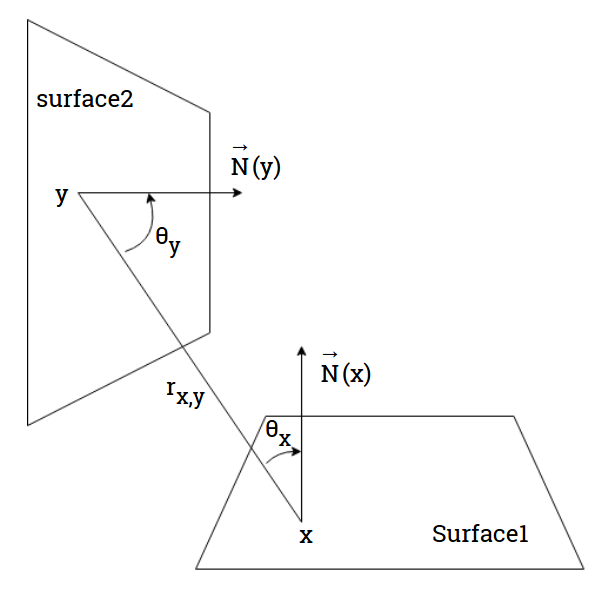
\includegraphics[width=0.4\linewidth]{xy.png}
\caption{Geometry in calculation of $K(x,y)$}
\label{fig:xytheta}
\end{figure}

\section {Radiosity Integral Equation}
Radiosity is governed by an non-homogeneous Fredholm integral equation of second kind (shown in Equation \ref{eq:NHFIEST}) which arises form more general problem of heat transfer known as rendering equation \cite{Kajiya} (see Appendix \ref{apen:derivationdegenerate}). In Equation \ref{eq:NHFIEST}, we solve integral equation for unknown function $\phi(x)$. 
\begin{equation} \label{eq:NHFIEST}
\phi(x)=f(x)+\lambda\int_{M^2} K(x,y)\phi(y)dy\quad x,y \in M^2
\end{equation}
In radosity, problem can be casted to integral equation shown in eq. (\ref{eq:genrie}). One way to relate equation with radiosity problem is that the radiosity $B(x)$ at point $(x)$  is sum of emitted radiosity $E(x)$ and reflected radiosity $p(x)K(x,y)B(y)$ which is received from all (integral) the points $y \in M^2$,  domain of all the surfaces in the scene.\\

\begin{equation} \label{eq:genrie}
B(x)=E(x)+p(x)\int_{M^2}K(x,y)B(y)dy
\end{equation}
In eq. (\ref{eq:genrie}) the integral is over all the points in domain of all  the surfaces $M^2$ in the scene. The kernel of integral equation is $p(x)K(x,y)$, which is calculated from geometry of input scene. Thus we can solve radiosity integral equation to solve radiosity problem.


% The parameters c and d takes value depending on  the scene. For 2D scenes, a scene consisting of lines instead of surfaces, d takes the value 1 and c takes the value 1/2 and the domain of the points is 1D. In the case of 3D scenes d takes the value 2 and c takes the value 1/$\pi$. From this point onwards we will refer to points by x and depending on the context (1D or  2D) it will be defined. The eq. (\ref{eq:3drie}) can be written as shown in eq. (\ref{eq:genrie})\\\\
% {\bf show equation (3)}
% \begin{equation} \label{eq:genrie}
% B(x)=E(x)+P(x)\int K(x,y)B(y)dy\\\\
% \end{equation}
\section{Analytical and Numerical Solution}
In literature lot of methods where developed to solve the non-homogeneous Fredholm integral of second kind \cite{iesurvey} \cite{ie}. In particular, if the kernel K is degenerate, one can find exact solution of the radiosity integral equation analytically \cite{ie}. But for even simple 2D  scene (flatland, see Chapetr \ref{ch:waveletprojection}), the kernel is non-degenerate. If analytical solution is not possible then one can solve the problem by approximation methods like Collocation Method, Galerkin Method \cite{iesurvey} \cite{ie}. We therefore use finite element methods(FEM) to compute approximate solution. We write unknown radiosity function as linear combination of basis function. Thus the problem get casted to system of linear equations which can be solved and approximate solution can be computed. In other words we solve the problem in finite dimensional function space instead of $L^2$ space, space of finite energy function. This method is also known as projection methods, more on these is discussed in next section.


    

\chapter{\label{ch:projection}Projection methods for radiosity problem}
In chapter \ref{ch:problemformulatio} we saw that problem of radiosity was casted to integral equation but it is very difficult to solve the integral equation analytically due to geometry of scene. We can use projection methods to find approximate solution. We first start with projecting the unknown radiosity function and integrate(operate kernel) on the projected function. After that we cast radiosity problem with system of linear equations. \\

\section{Projecting Radiosity Function}
We are working with linear operator (integral operator) defined on space of unknown function $B(x)$ we must first consider bases for this spaces. In general we will be dealing with functions of finite energy, i.e. functions
in the linear vector space $L^2$ . There are many possible bases for
this space. Consider some primal basis $\{N_i \}_{i{\bf belongs to}Z}$ . This set must contain infinitely many functions since $L^2$ is infinite dimensional.
By definition, every function $B{\bf belongs to}L^2$ can be written as a lin-
ear combination of the basis functions $B(x) = \sum _i b_i N_i(x)$ for
some coefficients $b_i$ . In order to find the coefficients of a given
function we need an inner product on $L^2$ . The inner product of
two functions F and G is defined as $<F, G> = \int F(x) G(y) ds$.
Throughout we will denote functions by capital letters. Their expansion coefficients with respect to a basis will be small letters
with indices as subscripts. When denoting functions we will often
drop the argument x (or y).
Given a function B and a set of basis functions $N_i$ , one way
of finding the coefficients of B with respect to this basis is by
performing inner products against the dual basis functions $N{\bf tilde}_i$
dual functions form a basis for the same space, and are defined
through the property\\
$<N_i,N{\bf tilde}_j>=\delta_{ij}$
where $\delta_{ij}$ is the Kronecker Delta. Using the duals we can write
the expansion of a function with respect to a basis as\\

$B(x) = \sum_ib_iN_i(x)= \sum_i<B,N_i>N_i(x)$\\

Now consider a linear operator defined on L 2 . One example is
integration against a kernel function, which is a linear operator since integration is linear. In particular we consider the radiosity
integral equation, which can be written as a linear operator\\

$B=E+KB$\\

where $KB(x) = \int K(x, y)B(y)dy$. Since K is a linear operator it
is fully described by its action on our chosen basis. Intuitively we
can write this as an infinite sized matrix. The columns of the matrix K are given by $KN_j$ . The coefficients of these columns with
respect to our basis can be found by taking inner products with
the dual functions. Thus the entries in the matrix representation
of K are given by\\

$K_{i,j}=<KN_j,N{\bf tilde}_i>=\int \int K(x,y)N_j(y)N{\bf tilde}_i(x)$\\

with this we can write radiosity integral equation as an infinite sized matrix equation\\

$(I-K)B=E$\\

{\bf Show countably finite thing \\ and also show the difference between space and basis for that space}\\

in next section we introduce wavelets and the wavelet basis
\\\\
    \chapter{\label{ch:wavelets}Wavelets}
Wavelet constitute a family of functions constructed from dilation and translation of a single function called the mother wavelet. When the dilation parameter a and the translation parameter b vary continuously, we have the following family of continuous wavelets as [Boggess]\\

$\psi_{a,b}(x) = {|a|}^{-1} \psi(\frac {t-b}{a})
,   \hspace{0.2cm} a,b \in R, a \neq 0.
$\\

If we restrict the parameters $a$ and $b$ to the discrete values as $a = a_0 ^-k, \\b = n b_0 a_0^{-k}$, where $a>1,b>0$ and $n$, and $k$ are positive integers, we have the following of discrete wavelets:\\

$\psi_n,k(x) = |a|^\frac{k}{2} \psi(a_0^k t - nb_0)$ ,\\
 which from a wavelet basis for $L^2(R)$. In particular, when $a_0 = 2$ and $b_0 = 1$ then $\psi_n,k (x)$ forms an orthonormal basis [Boggess].
 
 {\bf describe all the wavelet i am going to use like haar, llmw, qlmw, CAS 
 plots twoscale elation and vanishing moments and basis set}
 
 
    \chapter{\label{ch:waveletprojection}Wavelet radiosity}
In previous Chapters projection methods and wavelet has been described. Now we describe the use of wavelet basis for projection method and its advantages. 
We first start with the use of wavelet basis for expanding our unknown radiosity function B(x) as linear combination of wavelet basis.\\

$B(x) = b_{\phi_0}\phi_0(x)+\sum_{i,j}^{\inf,\inf}b_{\psi_{i,j}}\psi_{i,j}(x)$\\,
where $b_{\phi_0}$ and $b_{\psi_{i,j}}$ coefficients are inner products\\
$b_{\psi_{i,j}}=<B(x),psi_{i,j}(x)>$
From inner product point of view, we find that the small coefficients occur because wavelet functions have vanishing moments.
\underline{ define vanishing moments}\\

Different wavelet have different vanishing moments. For example Haar wavelet have one vanishing moment. Due to this a function which is nearly constant over the support of wavelet basis function will have coefficient value near 0 corresponding to that wavelet basis function. Similarly linear Legendre multi-wavelets have two vanishing moment, hence function nearly linear will have near 0 coefficient corresponding to that wavelet basis function. This is the advantage of using wavelet basis over box function as basis.\\

Once we project the radiosity function into wavelet basis we need to operate the integral on the projected as discussed in Chapter \ref{ch:projection}.
\begin{figure}[tbh]
\centering{}
\captionsetup{justification=centering}
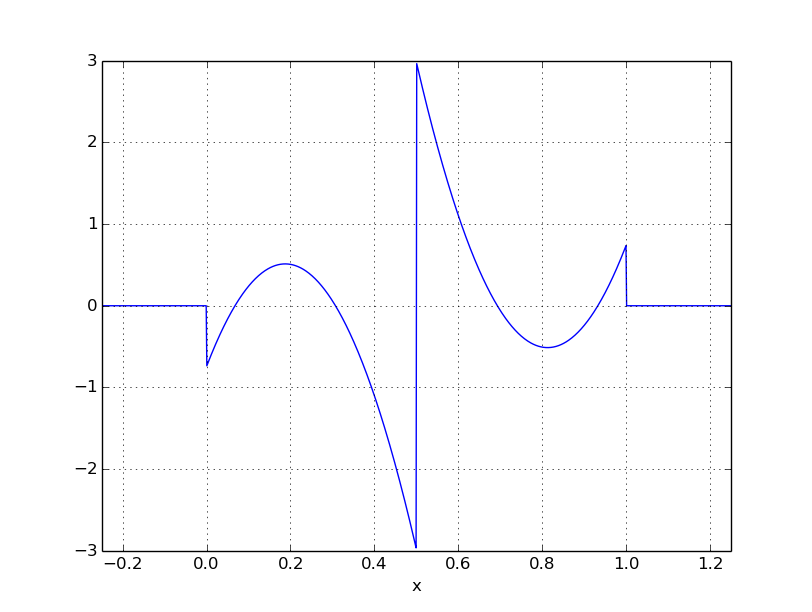
\includegraphics[width=3in]{qlmwpsi2.png}
\caption{\label{fig:f1scene}flatland1 scene: Two parallel segment of length $1$ and $\frac{1}{4}$ apart }
\end{figure}

\begin{figure}[tbh]
\centering{}
\captionsetup{justification=centering}
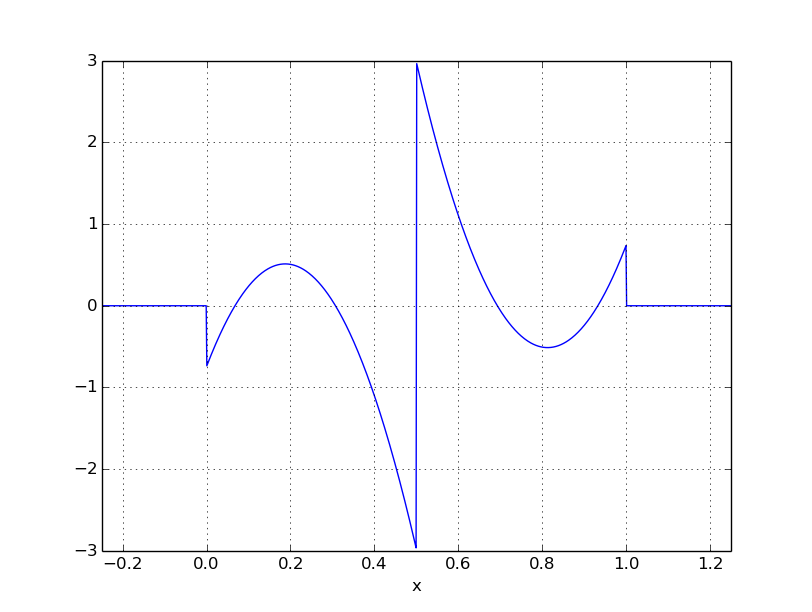
\includegraphics[width=3in]{qlmwpsi2.png}
\caption{\label{fig:f2scene}flatland1 scene: Two parallel segment of length $1$ and $\frac{1}{4}$ apart }
\end{figure}
Consider a 2D scene consisting of the two parallel line segment of length $1$ meter and at distance of $0.25$ meter (see Figure \ref{fig:f1scene}. We divided each segment into 64 equal parts and assume that radiosity function over each part is constant function. Thus we have space of piecewise constant function over the domain of each segment. One of the basis for this space is dilated and translated Haar scaling function (see Chapter \ref{ch:wavelets}). As we have discussed in Chapter \ref{ch:wavelets}, we have alternative basis for the space. This basis is Haar wavelet basis(see Chapter \ref{ch:wavelets}). Figure \ref{fig:haarscalesparsef1} shows the radiosity matrix $K$ with element $K_{i,j}$ obtaned by Equation \ref{eq:kijcalc}, when Haar scaling functions were used for projection. Figure \ref{fig:haarscalesparsef1} shows the radiosity matrix $K$, when Haar wavelet functions were used for projection. Note that each circle represent element. Value of element is proportional to radius of circle corresponding to that element. We can see that just changing the basis of approximation space to wavelet basis, we get very sparse matrix. Some of the elements can be replaced with zero, since many of the elements have value very near to zero. By doing so we will get increased error in projection. But error is very small as compared to sparsity we get after doing so. This sparsity is result of vanishing moments of wavelet. More the vanishing, more will be the sparsity.\\




{\bf explain about the kernel sparsity of wavelet projection }\\
Figure 

\begin{figure}[tbh]
\centering{}
\captionsetup{justification=centering}
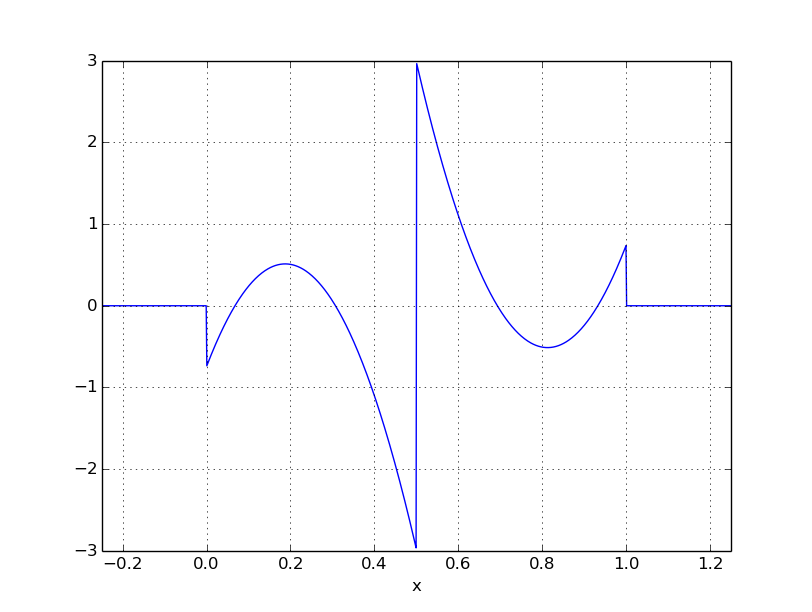
\includegraphics[width=3in]{qlmwpsi2.png}
\caption{\label{fig:haarscalesparsef1}flatland1 with $dist=0.25$ kernel sparsity plot haar scale, radius of circle is proportional to value of element}
\end{figure}
\begin{figure}[tbh]
\centering{}
\captionsetup{justification=centering}
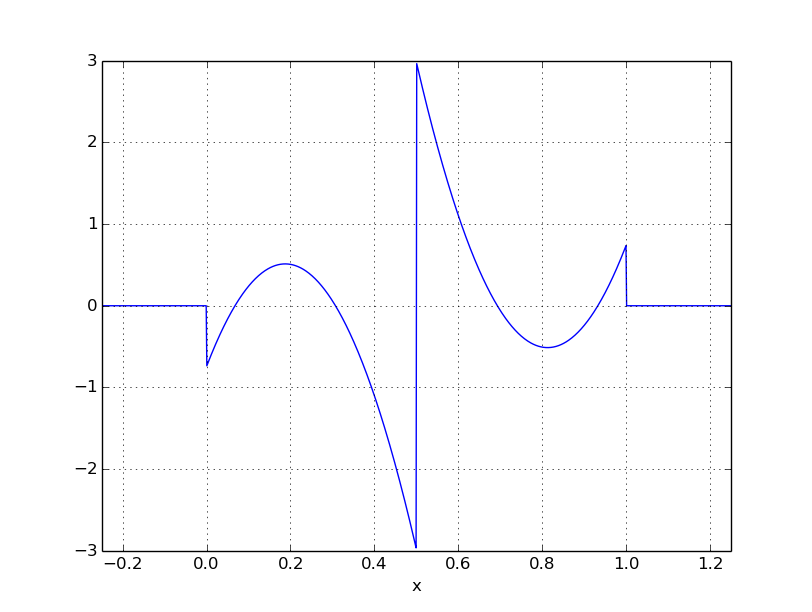
\includegraphics[width=3in]{qlmwpsi2.png}
\caption{\label{fig:haarwaveletsparsef1}flatland1 with $dist=0.25$ kernel sparsity plot haar wavelet}
\end{figure}

Consider another 2D scene consisting of two line segment of length $1$ perpendicular to each other (see Figure \ref{fig:f2scene}. One can see from figure \ref{fig:haarscalesparsef2} and \ref{fig:haarwaveletsparsef2} that similar results are obtained for different 2D scene.

\begin{figure}[tbh]
\centering{}
\captionsetup{justification=centering}
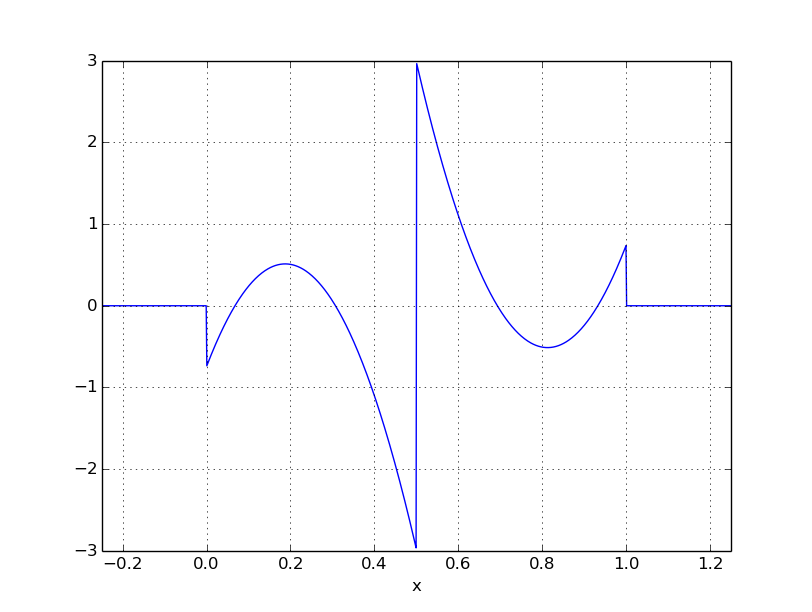
\includegraphics[width=3in]{qlmwpsi2.png}
\caption{\label{fig:haarscalesparsef2}flatland1 with $dist=0.25$ kernel sparsity plot haar scale, radius of circle is proportional to value of element}
\end{figure}
\begin{figure}[tbh]
\centering{}
\captionsetup{justification=centering}
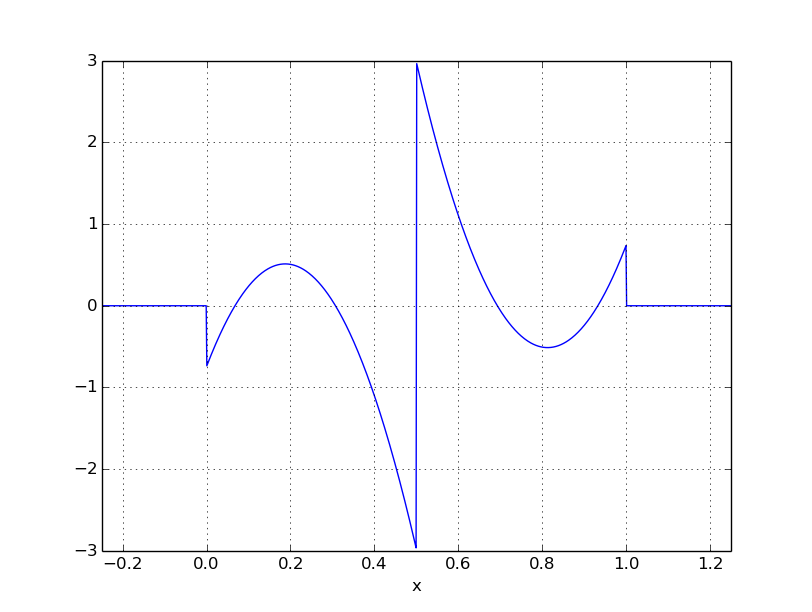
\includegraphics[width=3in]{qlmwpsi2.png}
\caption{\label{fig:haarwaveletsparsef2}flatland1 with $dist=0.25$ kernel sparsity plot haar wavelet}
\end{figure}

\section{Three Dimensional Radiosity and Implementation}
For understanding advantages of wavelet basis we selected 2D scenes. But for 3D scene we need to have 2D basis defined over domain of all 2D surfaces of 3D scene. One simplest way to get 2D wavelet is tensor product of 1D basis. Thus 3D radiosity problem can be solved using projection method with 2D wavelet basis. Coefficients are calculated using Gauss quadrature \cite{stoer}. Thus we need to calculate 4D integral to find coefficient of 4D radiosity matrix $K$. A $p$ point  Gauss-Legendre rule can calculate an accurate integral for polynomials of order up to  $2p-1$.

In next chapter, Chapter \ref{ch:experimentandresult}, we tested wavelet basis with more 2D scenes and also discussed results of 3D radiosity scenes.




\begin{figure}[tbh]
\centering{}
\captionsetup{justification=centering}
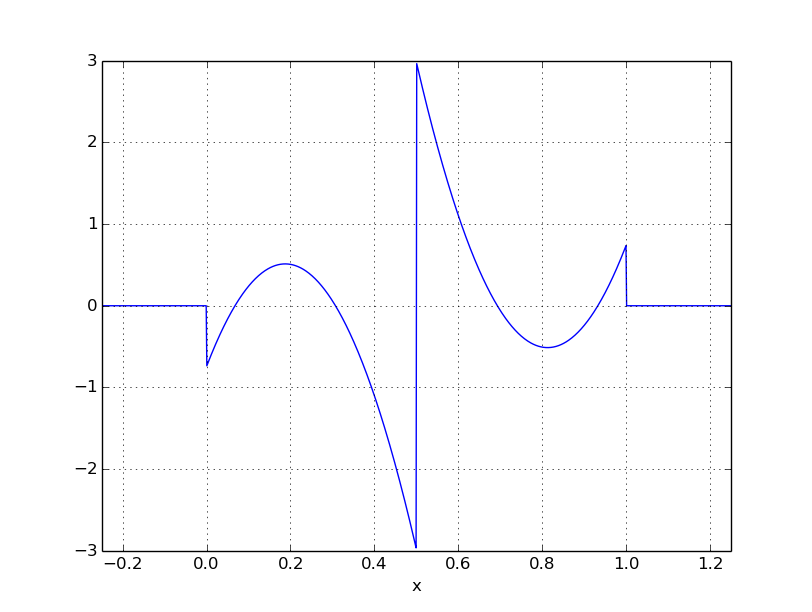
\includegraphics[width=3in]{qlmwpsi2.png}
\caption{\label{fig:replacethis7}flatland1 with $dist=0.25$ kernel sparsity plot llmw wavelet}
\end{figure}

\begin{figure}[tbh]
\centering{}
\captionsetup{justification=centering}
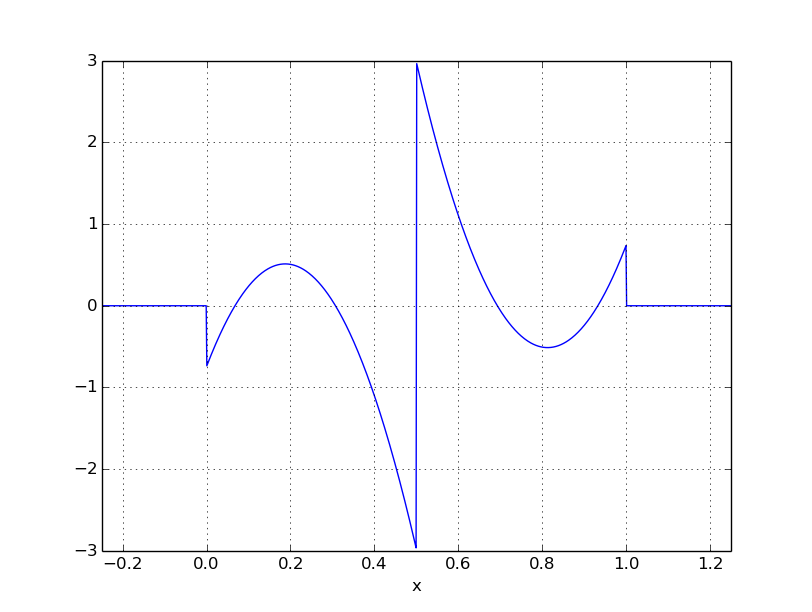
\includegraphics[width=3in]{qlmwpsi2.png}
\caption{\label{fig:replacethis8}flatland1 with $dist=0.25$ kernel sparsity plot qlmw wavelet}
\end{figure}
\underline{discuss about m2 and m3 aswell, also tell about advantage of sparse matrix}

\begin{figure}[tbh]
\centering{}
\captionsetup{justification=centering}
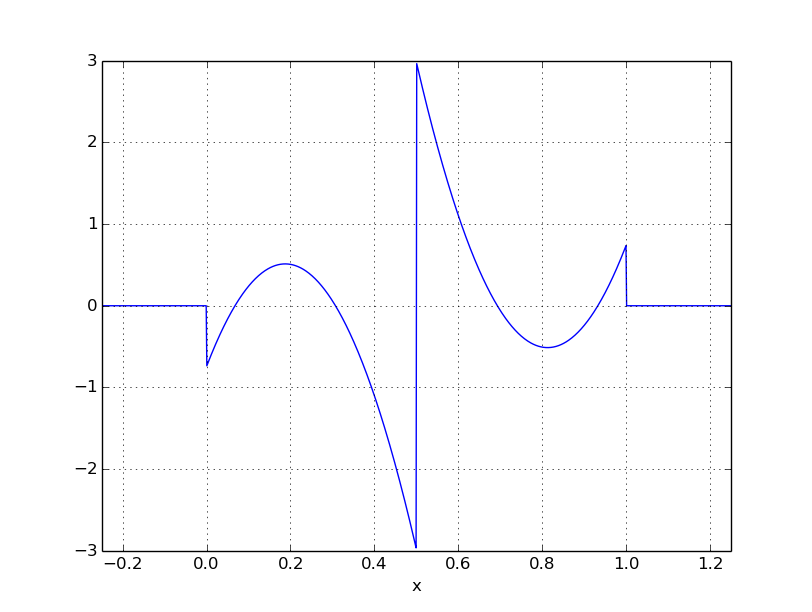
\includegraphics[width=3in]{qlmwpsi2.png}
\caption{\label{fig:replacethis10}flatland2  kernel sparsity plot  llmw wavelet}
\end{figure}

\begin{figure}[tbh]
\centering{}
\captionsetup{justification=centering}
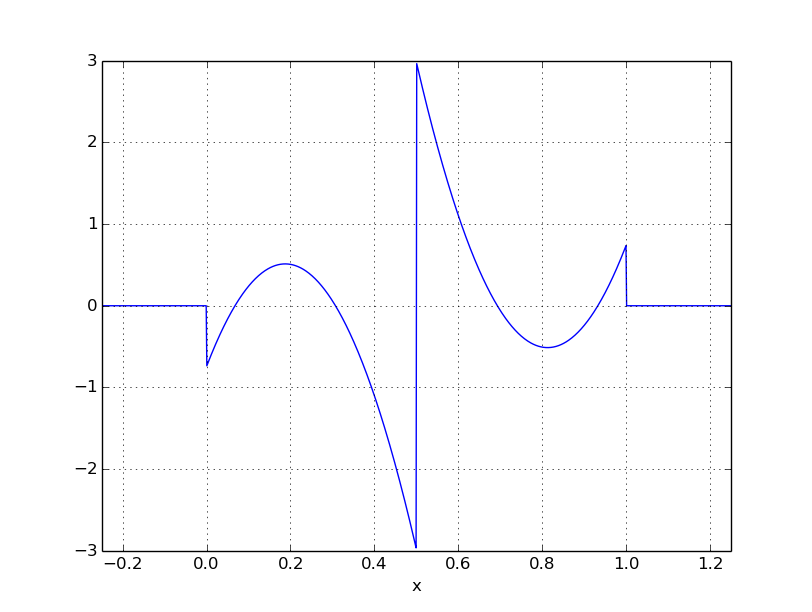
\includegraphics[width=3in]{qlmwpsi2.png}
\caption{\label{fig:replacethis11}flatland2 kernel sparsity plot qlmw wavelet}
\end{figure}

{\bf expalin about 2D and 4d wavelet function (tensor product)}
    \chapter{\label{ch:experimentandresult}Experiments and results}
In this chapter a comparison of wavelets discussed in chapter  \ref{ch:wavelets} is analyzed with characteristic scenes in 2D (flatland) and 3D. Such a comparison can never be exhaustive due to the heterogeneous nature of input scenes. Therefore scenes with different kind of kernels has been chosen for comparison of performance of the wavelets. We first discuss kernels for which we have the exact analytical solution of the integral equation. Then we test and compare the wavelets the 2D scenes knows as flatland scenes. Flatland scenes are selected mainly to analysis and understanding different aspects of using wavelet basis for radiosity. Results of using the different wavelets with 3D scenes are also discussed at the end this chapter. \\

% {\bf Ground truth comparison}\\
\section{Integral Equation with degenerate kernel}
For comparing the approximate solution with exact ground truth we chose kernels which are classified as degenerate kernels. Degenerate kernels are kernels which can be expanded in the form shown in Equation (\ref{eq:kxydegen})
\begin{equation} \label{eq:kxydegen}
K(x,y) = \sum\limits_{i=1}^na_i(x)b_i(y) \\ 
\end{equation}
An integral equation with degenerate kernel can be solved by changing the order of integral and summation after substituting expanded kernel. See a
Appendix \ref{apen:derivationdegenerate} for analytical solution of non-homogeneous Fredholm IE of second kind. 

We took kernel 
\begin{equation}\label{eq:kernelanalytical}
 K(x,y)=x^2+xy, \quad x,y \in [0,1]
\end{equation}
for comparing different wavelets with the ground truth solution 
\begin{equation}\label{eq:solutinoanalytical}
    B(x)=\frac{66}{23}x^2+\frac{42}{23}x+1
\end{equation}
 of the IE shown in Equation \ref{eq:genrie}
 We substitute this kernel in Equation \ref{eq:genrie} to get IE equation,
\begin{eqnarray} \label{eq:analytical}
B(x)=E(x)+\int\limits_0^1 K(x,y)B(y) dy \\
 = E(x)+\int\limits_0^1 (x^2+xy )B(y) dy
\end{eqnarray}

We compare wavelets by calculating error in the projection of kernel $K(x,y)$ and error in solution $B(x)$. The metric used for comparison is relative error as shown in Equation \ref{eq:Krelerr}. It is a ratio of $L^2$ norm of error $(K(x,y)-\hat{K}(x,y))$ to $L^2$ norm of kernel. The integration is over entire domain of x and y. Where $\hat{K}(x,y)$ is approximation of $K(x,y)$ in space spanned by chosen wavelet.
\begin{equation} \label{eq:Krelerr}
\text{relative  error}=\frac{\int\int \,(\,K(x,y)-\hat{K}(x,y)\,)^2  \,dy \, dx}{\int\int \,K(x,y)^2  \,dy \, dx}
\end{equation}
The purpose of selecting degenerate kernel is to make sure that the implemented algorithm works properly and algorithm is fit for testing the wavelets with the scenes for which we do not have the ground truth analytical solution. Note that the kernels discussed in this section does not describe any real world scene. 

Approximate solution is calculate using projection method shown in Chapter \ref{ch:waveletprojection}. Figure \ref{fig:ahaar4}, \ref{fig:ahaar4}, \ref{fig:allmw2}, \ref{fig:allmw4}, \ref{fig:aqlmw2}, shows the approximate solution and error function with different wavelets without thresholding(replacing negligible elements  with value 0). This shows that as we increase n, error reduces and as we increase vanishing moments of wavelet from Haar wavelet to QLMW error decreases. Above two result shows that to decrease error in  solution either n or order basis function has to be increased. Also for QLMW error is zero for all $n$ because $K(x,y)$ lies in space spanned by QLMW basis.



\begin{figure}[h!]
\centering{}
\captionsetup{justification=centering}
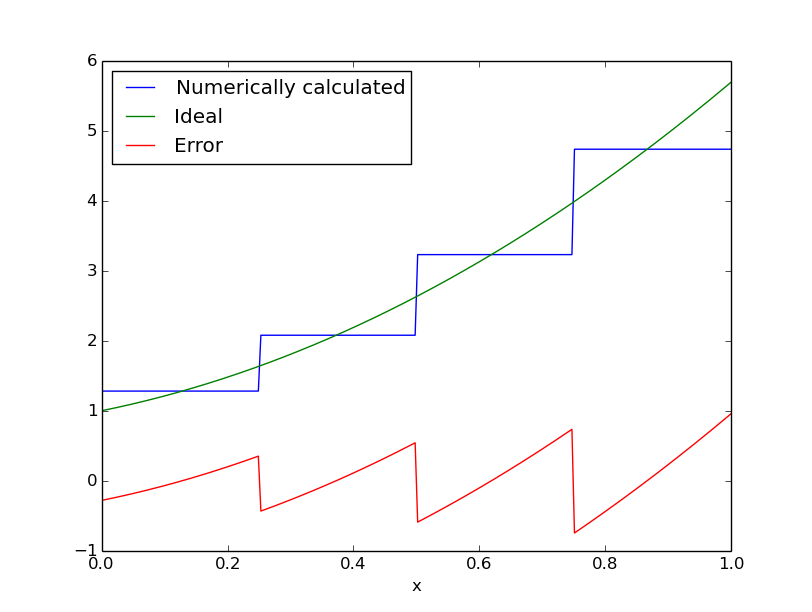
\includegraphics[width=5in]{ahaar4.png}
\caption{\label{fig:ahaar4}Haar wavelet: Solution and Error in solution of Equation \ref{eq:analytical} with $n=4$}
\end{figure}

\begin{figure}[h!]
\centering{}
\captionsetup{justification=centering}
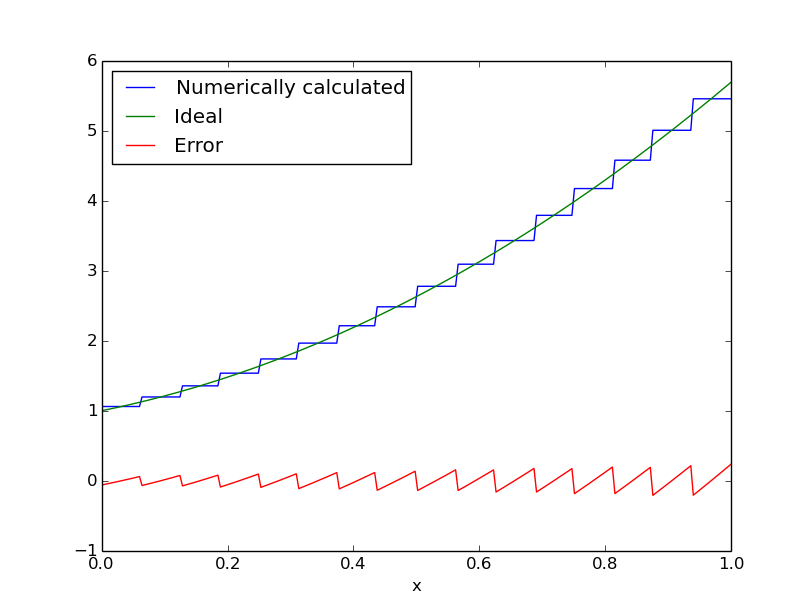
\includegraphics[width=5in]{ahaar16.png}
\caption{\label{fig:ahaar16}Haar wavelet: Solution and Error in solution of Equation \ref{eq:analytical} with $n=16$}
\end{figure}
\begin{figure}[h!]
\centering{}
\captionsetup{justification=centering}
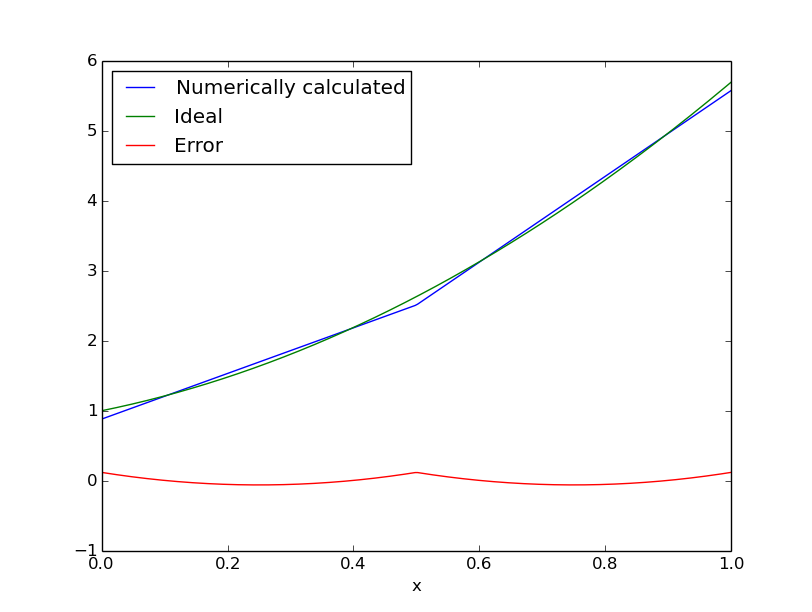
\includegraphics[width=5in]{allmw2.png}
\caption{\label{fig:allmw2}LLMW wavelet: Solution and Error in solution of Equation \ref{eq:analytical} with $n=2$}
\end{figure}
\begin{figure}[h!]
\centering{}
\captionsetup{justification=centering}
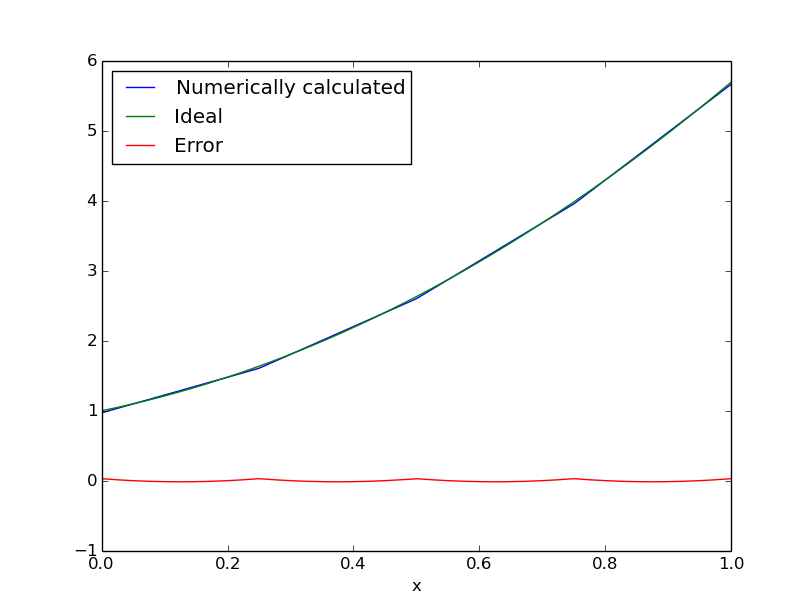
\includegraphics[width=5in]{allmw4.png}
\caption{\label{fig:allmw4}LLMW wavelet: Solution and Error in solution of Equation \ref{eq:analytical} with $n=4$}
\end{figure}


\begin{figure}[h!]
\centering{}
\captionsetup{justification=centering}
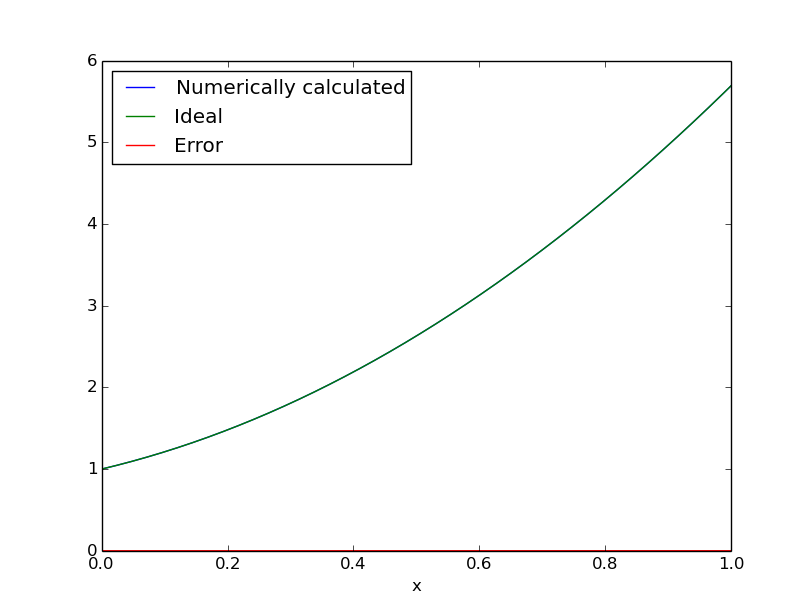
\includegraphics[width=5in]{aqlmw2.png}
\caption{\label{fig:aqlmw2}QLMW wavelet: Solution and Error in solution of Equation \ref{eq:analytical} with $n=2$}
\end{figure}

As we have tested implemented algorithm with 2D kernels, we also have tested algorithm with 4D kernels as shown below,
\begin{equation}\label{eq:kernelanalytical4d}
 K(x_1,y_1,x_2,y_2)=x_1 y_1 x_2 y_2, \quad x_1,y_1,x_2,y_2 \in [0,1]
\end{equation}
The analytical solution \ref{apen:derivationdegenerate} of the integral equation with above kernel,
\begin{eqnarray} \label{eq:analytical4d}
B(x_1,y_1)=E(x_1,y_1)+\int\limits_0^1 K(x_1,y_1,x_2,y_2)B(x_2,y_2) dy \\
 = E(x_1,y_1)+\int\limits_0^1 (x_1y_1x_2y_2)B(x_2,y_2) dy
\end{eqnarray}
is,
\begin{equation}\label{eq:solutinoanalytical4d}
    B(x_1,y_1)=1+\frac{9}{32}x_1y_1
\end{equation}

The comparison of different wavelet is done in similar way as in 2D kernel case seen above. Figure \ref{fig:4d_analytical_haar_2}, \ref{fig:4d_analytical_llmw_2} and \ref{fig:4d_analytical_qlmw_2} shows the comparison of solution with $m=0,1,2$ and $n=2$. Note that numerical solution with $m=1,2$ is same as analytical solution as the approximate finite space is same as the space of original problem. Figure \ref{fig:4d_analytical_haar_4} shows the solution with $m-0$ and $n=4$. 

\begin{figure}[h!]
\centering{}
\captionsetup{justification=centering}
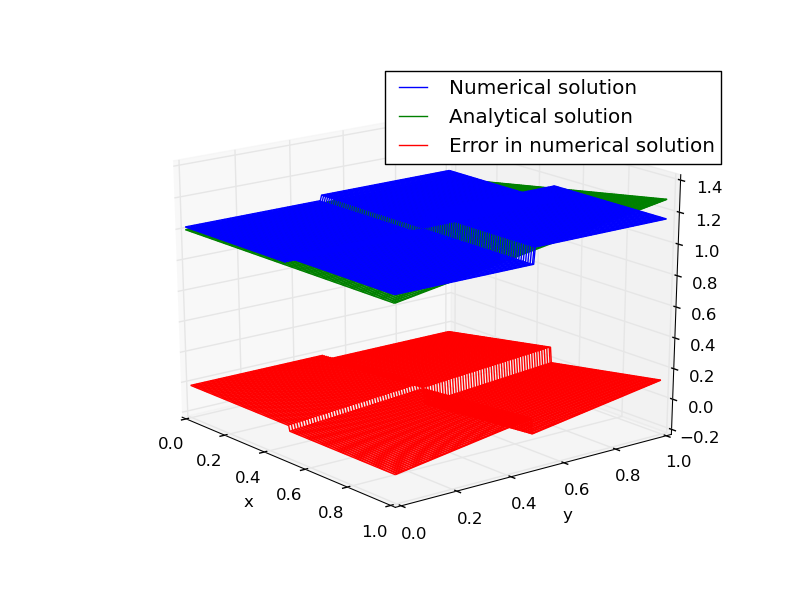
\includegraphics[width=5in]{4d_analytical_haar_2.png}
\caption{\label{fig:4d_analytical_haar_2}Haar wavelet: Analytical and Numerical solution of equation \ref{eq:analytical4d} with $n=2$}
\end{figure}



\begin{figure}[h!]
\centering{}
\captionsetup{justification=centering}
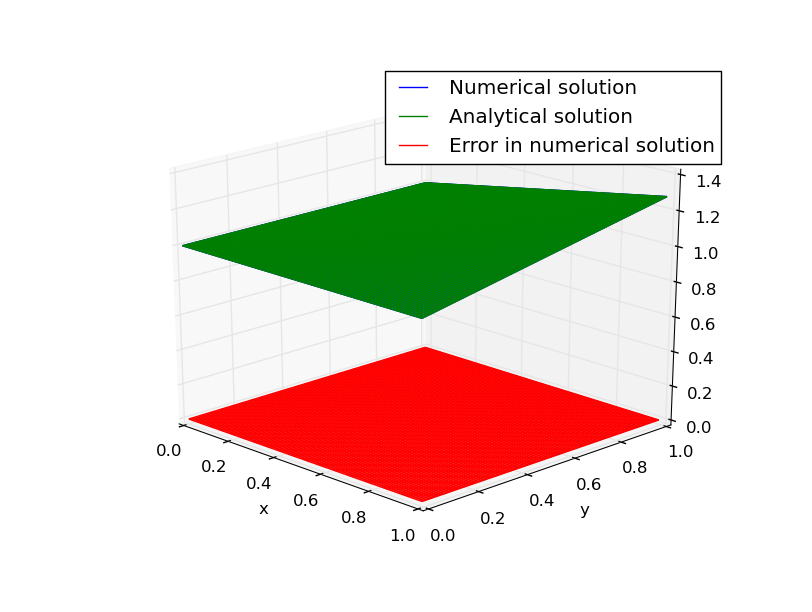
\includegraphics[width=5in]{4d_analytical_llmw_2.png}
\caption{\label{fig:4d_analytical_llmw_2}LLMW wavelet: Analytical and Numerical solution of equation \ref{eq:analytical4d} with $n=2$}
\end{figure}


\begin{figure}[h!]
\centering{}
\captionsetup{justification=centering}
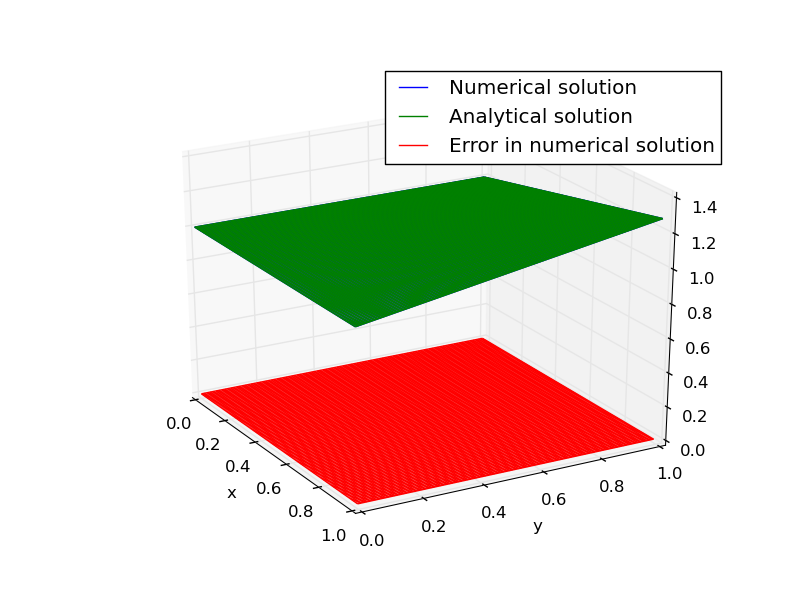
\includegraphics[width=5in]{4d_analytical_qlmw_2.png}
\caption{\label{fig:4d_analytical_qlmw_2}QLMW wavelet: Analytical and Numerical solution of equation \ref{eq:analytical4d} with $n=2$}
\end{figure}

\begin{figure}[h!]
\centering{}
\captionsetup{justification=centering}
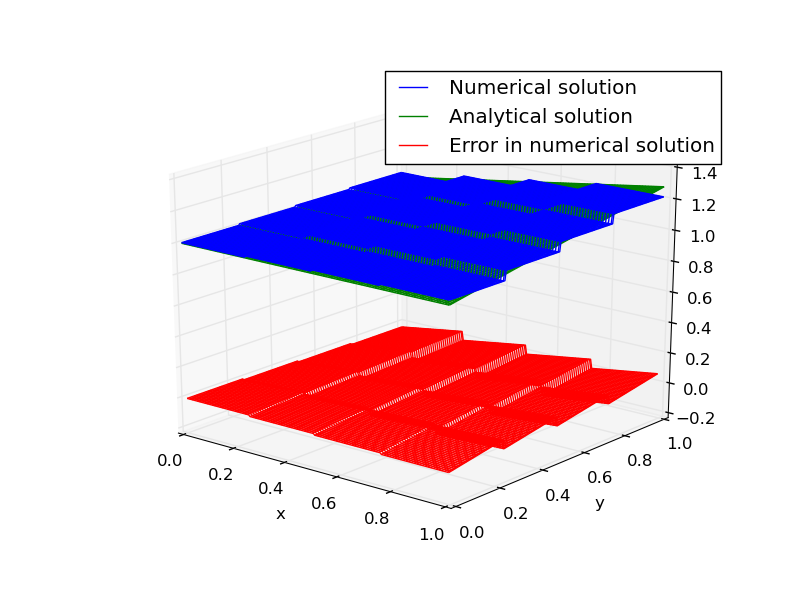
\includegraphics[width=5in]{4d_analytical_haar_4.png}
\caption{\label{fig:4d_analytical_haar_4}Haar wavelet: Analytical and Numerical solution of equation \ref{eq:analytical4d} with $n=4$}
\end{figure}


\section{Flatland radiosity}
In this section we first discuss the relation of $n$ and $m$ with accuracy of projection of kernel for flatland scenes.  Then we discuss the comparison of different wavelets to solve radiosity for flatland scenes. Flatland is two dimensional world in which surfaces are one dimensional instead of two dimensional surfaces in three dimensional scene. We select flatland scenes for its simplicity and imaginability of kernel associated with scenes. Simplest flatland scene is scene with two parallel line segment of unit length each(see Figure \ref{fig:f1scene}) and scene with two line segment, of unit length each, perpendicular to each other(see Figure \ref{fig:f2scene}). 



Note that $x \in X$ and $y \in Y$ in above kernels. $K(x_1,x_2) = 0$ for $x_1,x_2 \in X$ as two points in a line segment do not interact directly, however they can interact indirectly through reflections from other line segment(see Figure \ref{fig:kernel}) for graphical representation of kernel of any two line segment in general. In other words interaction can take place only between two different planner surfaces(on lines in this context) on however, two points on single concave surface(or line) can interact directly.  The kernel $K(x,y)$ of flatland is calculated using \ref{eq:kernelflatland1}. We will refer to scene consist of parallel line segment as Flatland scene 1 and scene with two perpendicular line segment as Flatland scene 2. Kernel $K_1(x,y)$ for Flatland scene 1 is


\begin{figure}[tbh]
\centering{}
\captionsetup{justification=centering}
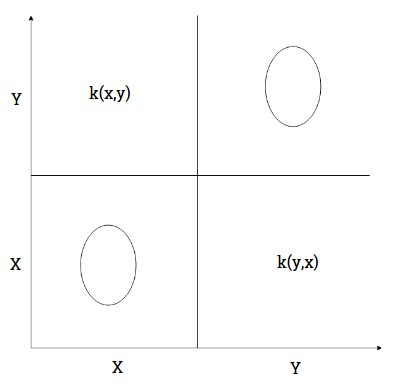
\includegraphics[width=5in]{kernel.png}
\caption{\label{fig:kernel}Flatland scene with two segments: Kernel, in general, with zero and non zero regions}
\end{figure}


\begin{eqnarray} \label{eq:kernelflatland1}
K_1(x,y)\quad=\frac{   \cos{\theta_x}  \cos{\theta_y}  }{    2\,r_{x,y}   }\quad\quad\quad\\
        =\frac{dist^2}{2((x-y)^2+dist^2)}
\end{eqnarray}
and kernel  $K_2(x,y)$ for flatland2 is

\begin{eqnarray} \label{eq:kernelflatland2}
K_2(x,y)\quad=\frac{\cos{\theta_x}\cos{\theta_y}}{2\,r_{x,y}} \quad\quad\quad\quad\quad\quad\quad\quad\quad\quad\\
\quad\quad\quad\quad\quad\quad\quad\quad\quad\quad\quad=\frac{(x+0.1)(y+0.1)}{2((x+0.1)^2+(y+0.1)^2)^{\frac{3}{2}}}\quad\quad\quad
\end{eqnarray}
We can change distance between two line segment in Flatland scene 1 to get different scene. As the distance decrease interaction between two segment increases. Figure \ref{fig:haarscalesparsef1} and \ref{fig:haarwaveletsparsef1} shows the kernel of Flatland scene 1 with $dist=0.25$. The kernel is non negative over entire domain. Also the interaction between two points is maximum when distance between them is less. \\

To see the relation of $n$ and $m$ with accuracy of projection of kernel for flatland scenes we select $m = 0,1,2$ and $n=4,8,16,32,64,128,256$. Figure  \ref{fig:nmtrend_f1} and \ref{fig:nmtrend_f2} conforms the relation of accuracy and n,m for flatland scenes.


\begin{figure}[tbh]
\centering{}
\captionsetup{justification=centering}
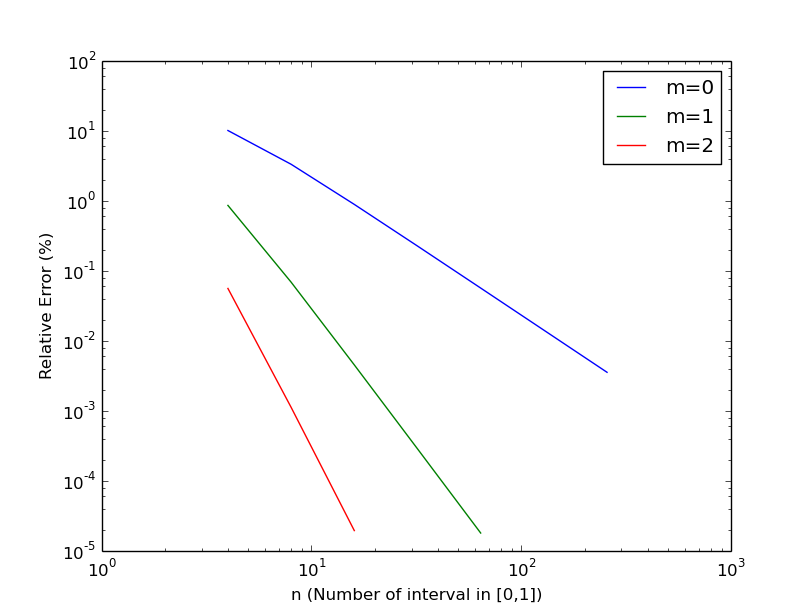
\includegraphics[width=5in]{nmtrend_f1.png}
\caption{\label{fig:nmtrend_f1}Relation of accuracy and n,m in projection of K(x,y) for Flatland Scene 1}
\end{figure}
\begin{figure}[tbh]
\centering{}
\captionsetup{justification=centering}
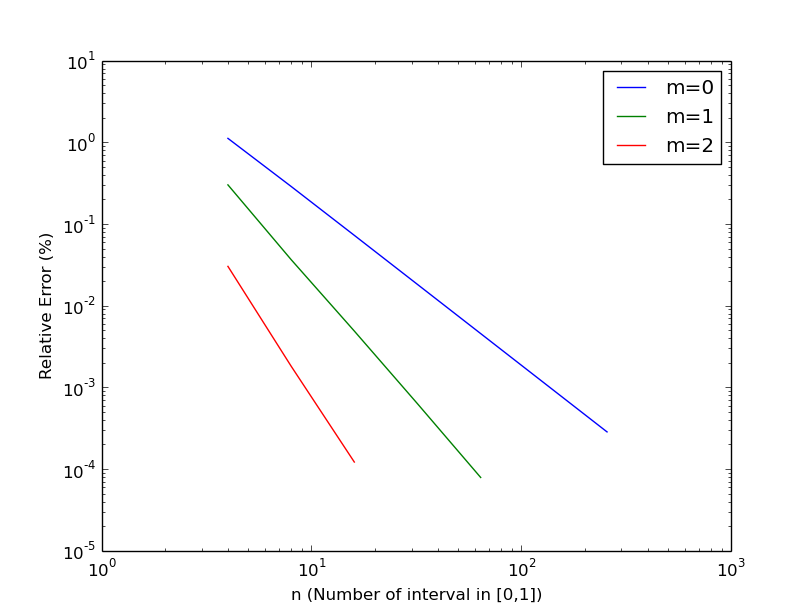
\includegraphics[width=5in]{nmtrend_f2.png}
\caption{\label{fig:nmtrend_f2}Relation of accuracy and n,m in projection of K(x,y) for Flatland Scene 2}
\end{figure}


Kernel is projected into space spanned by wavelet basis to get the sparse matrix of coefficient as shown in \ref{fig:haarwaveletsparsef1} \ref{fig:haarwaveletsparsef2}.




To see the sparsity of matrix we plot sorted elements of matrix. Figure \ref{fig:f1_0_25_haar_scale_distri_n_16} shows that coefficients of Haar wavelet basis are negligible for many basis functions as compared to Haar scaling functions. Similar result for LLMW and QLMW are shown in Figures \ref{fig:f1_0_25_llmw_scale_distri_n_16}, \ref{fig:f1_llmw_scale_distri_n_16}, \ref{fig:f1_0_25_qlmw_scale_distri_n_16}, \ref{fig:f1_qlmw_scale_distri_n_16}.
% {\bf show all the distance and and f2 comment on increase in element value vs decrease in distance also show poly-poly and wavelet-poly comparison for conclusion purpose }

      









\begin{figure}[tbh]
\centering{}
\captionsetup{justification=centering}
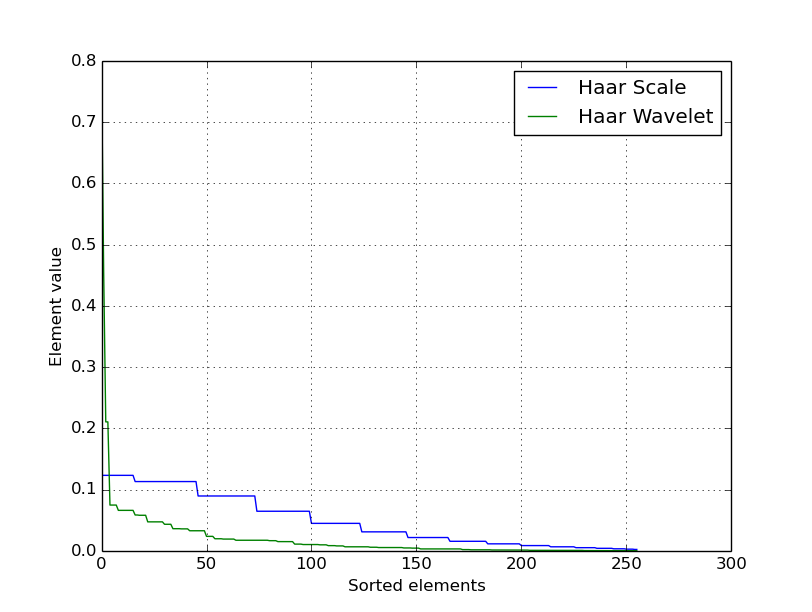
\includegraphics[width=5in]{f1_0_25_haar_scale_distri_n_16.png}
\caption{\label{fig:f1_0_25_haar_scale_distri_n_16}Distribution of kernel projection coefficients with Haar Wavelet and scale functions,$n=16$, for Flatland scene 1}
\end{figure}

\begin{figure}[tbh]
\centering{}
\captionsetup{justification=centering}
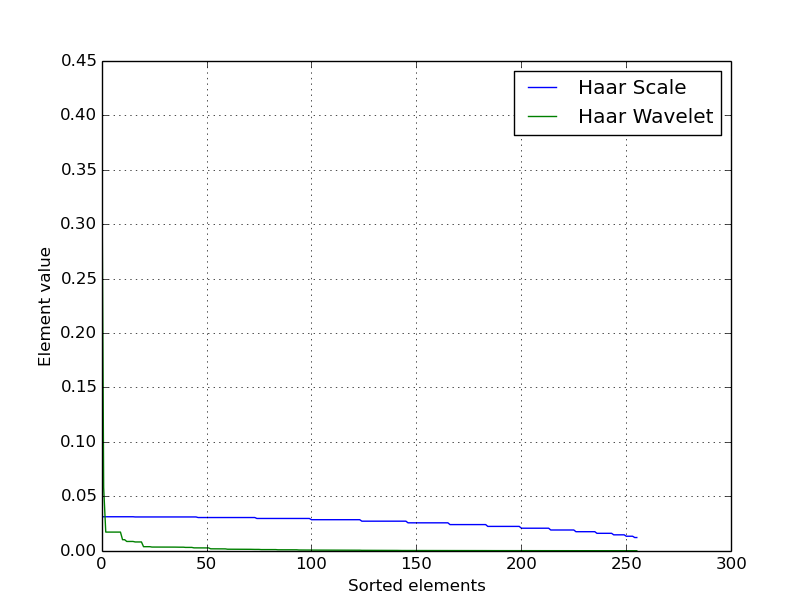
\includegraphics[width=5in]{f1_haar_scale_distri_n_16.png}
\caption{\label{fig:f1_haar_scale_distri_n_16}Distribution of kernel projection coefficients with Haar Wavelet and scale functions,$n=16$, for  Flatland scene 2}
\end{figure}

\begin{figure}[tbh]
\centering{}
\captionsetup{justification=centering}
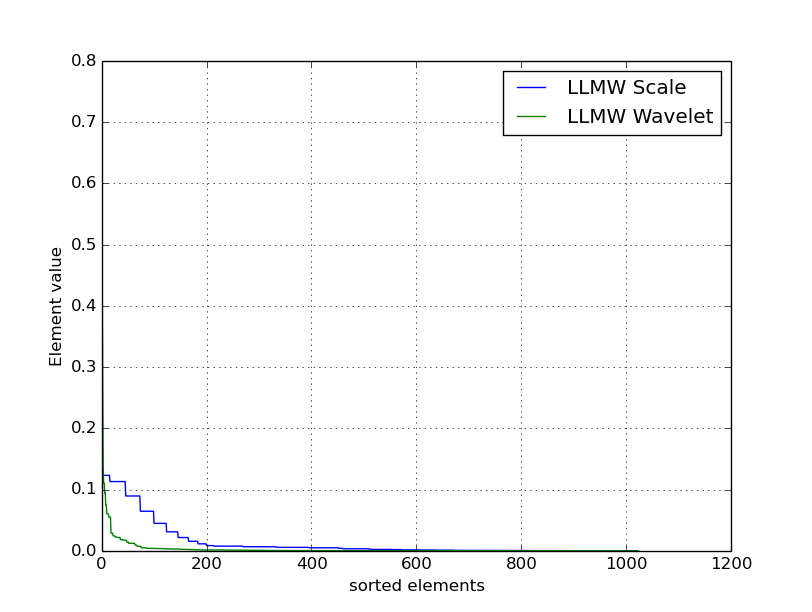
\includegraphics[width=5in]{f1_0_25_llmw_scale_distri_n_16.png}
\caption{\label{fig:f1_0_25_llmw_scale_distri_n_16}Distribution of kernel projection coefficients with LLMW Wavelet and scale functions,$n=16$, for Flatland scene 1}
\end{figure}

\begin{figure}[tbh]
\centering{}
\captionsetup{justification=centering}
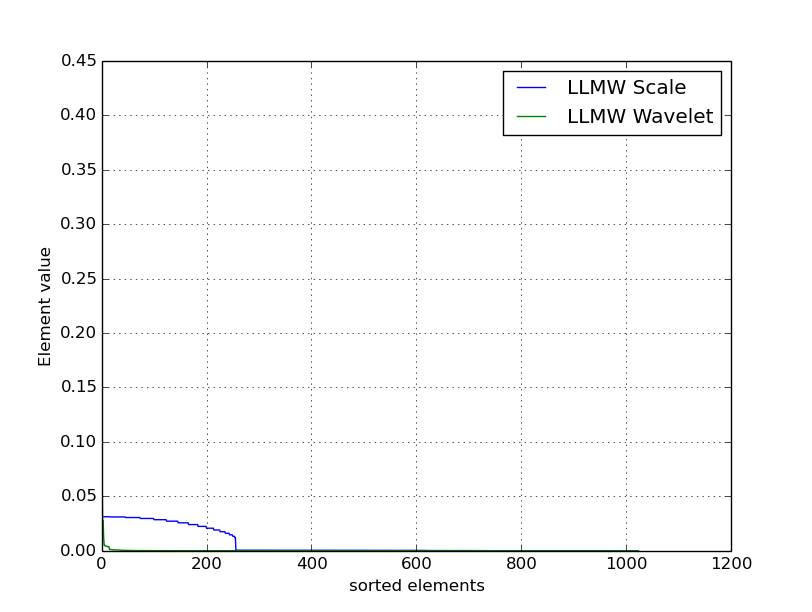
\includegraphics[width=5in]{f1_llmw_scale_distri_n_16.png}
\caption{\label{fig:f1_llmw_scale_distri_n_16}Distribution of kernel projection coefficients with LLMW Wavelet and scale functions,$n=16$, for  Flatland scene 2}
\end{figure}

\begin{figure}[tbh]
\centering{}
\captionsetup{justification=centering}
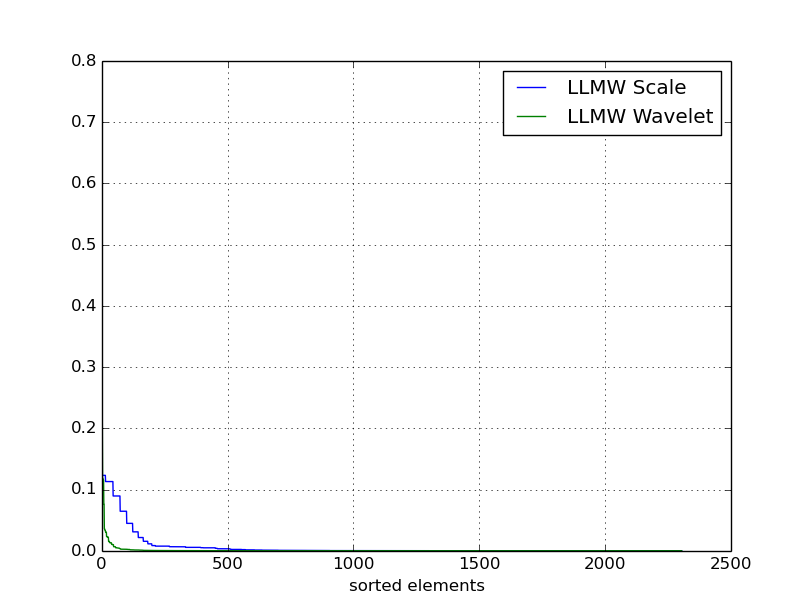
\includegraphics[width=5in]{f1_0_25_qlmw_scale_distri_n_16.png}
\caption{\label{fig:f1_0_25_qlmw_scale_distri_n_16}Distribution of kernel projection coefficients with QLMW Wavelet and scale functions,$n=16$, for Flatland scene 1}
\end{figure}

\begin{figure}[tbh]
\centering{}
\captionsetup{justification=centering}
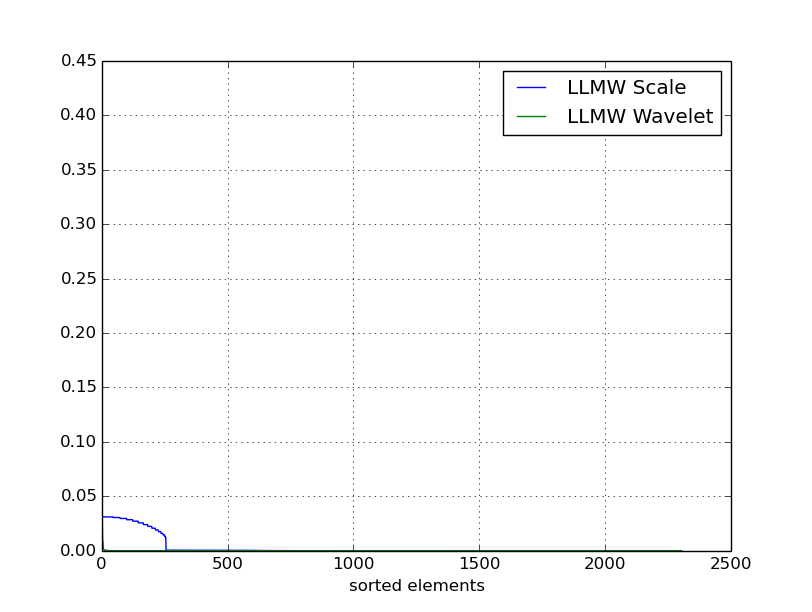
\includegraphics[width=5in]{f1_qlmw_scale_distri_n_16.png}
\caption{\label{fig:f1_qlmw_scale_distri_n_16}Distribution of kernel projection coefficients with QLMW Wavelet and scale functions,$n=16$, for  Flatland scene 2}
\end{figure}
Now we analyze the effect of setting all this negligible coefficients to zero by projecting kernel of Flatland scene 1 with Haar wavelet and scale basis with $n=256$. We select top $N$ elements from kernel projection while remaining are set to zero (thresholding). Figure \ref{fig:errorvstopnhaarwavelet}, \ref{fig:errorvstopnllmwwavelet} shows that error in projection of kernel after thresholding is much less in wavelet basis as compared to scaling function basis.


\begin{figure}[tbh]
\centering{}
\captionsetup{justification=centering}
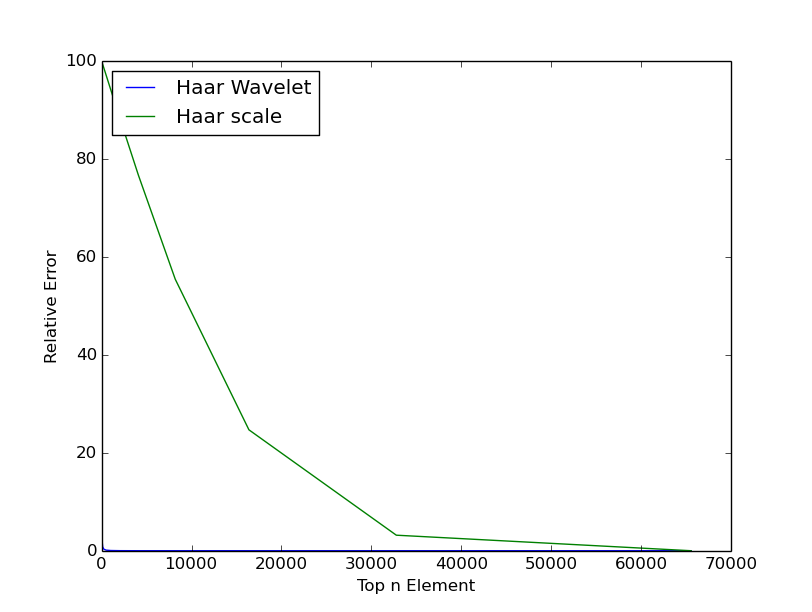
\includegraphics[width=5in]{topn256haarbothf1.png}
\caption{\label{fig:errorvstopnhaarwavelet}Error in projection,  keeping top $N$ element (set remaining to $0$) using both Haar Wavelet and Scale function with $n=256$ for  Flatland scene 1}
\end{figure}

\begin{figure}[tbh]
\centering{}
\captionsetup{justification=centering}
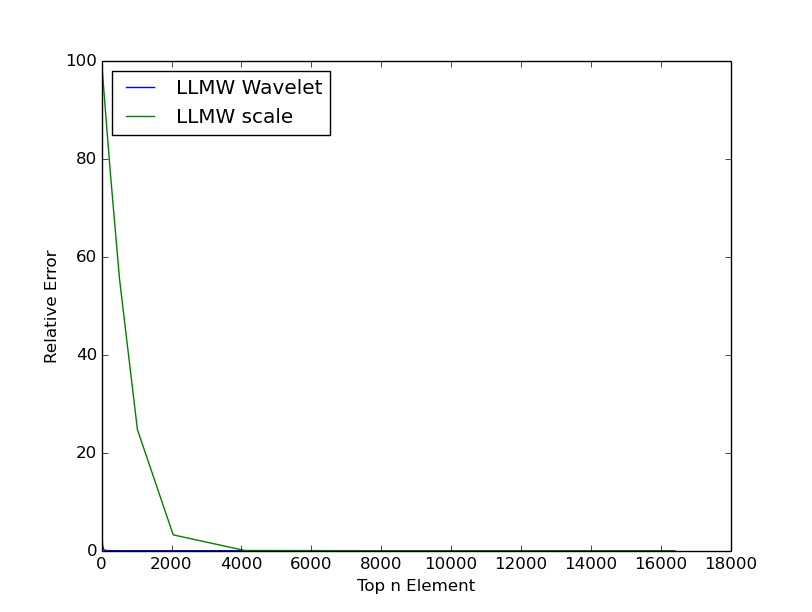
\includegraphics[width=5in]{64topnllmwf1.png}
\caption{\label{fig:errorvstopnllmwwavelet}Error in projection,  keeping top $N$ element (set remaining to $0$) using both LLMW Wavelet and Scale function with $n=64$ for  Flatland scene 1}
\end{figure}

% \begin{eqnarray} \label{eq:kernelflatland1}
% 

% \end{eqnarray}

% \begin{eqnarray} \label{eq:kernelflatland1}
% K_1(x,y)=\frac{\cos{\theta_x}\cos{\theta_y}}{2\,r_{x,y}}\\
% =\frac{dist^2}{2((x-y)^2+dist^2)}

% \end{eqnarray}

% and kernel  $K_2{x,y}$ for flatland2 is


% \begin{eqnarray} \label{eq:kernelflatland2}
% K_1(x,y)=\frac{\cos{\theta_x}\cos{\theta_y}}{2\,r_{x,y}} \quad x,y \in [0,1]
% \end{eqnarray}

Figure \ref{fig:f1_025_haar_scale_plot_n_16}, \ref{fig:f1_025_haar_scale_plot_n_16} and \ref{fig:f1_025_haar_scale_plot_n_16} shows the solution of flatland scene 1 with different $m=0,1,2$ and $n=16$.  We can see that $m=0$ gives blocky solution while $m=1,2$ gives relatively smooth solution.

\begin{figure}%
    \centering
    \subfloat[f1 025 haar scale b1 plot n 16]{{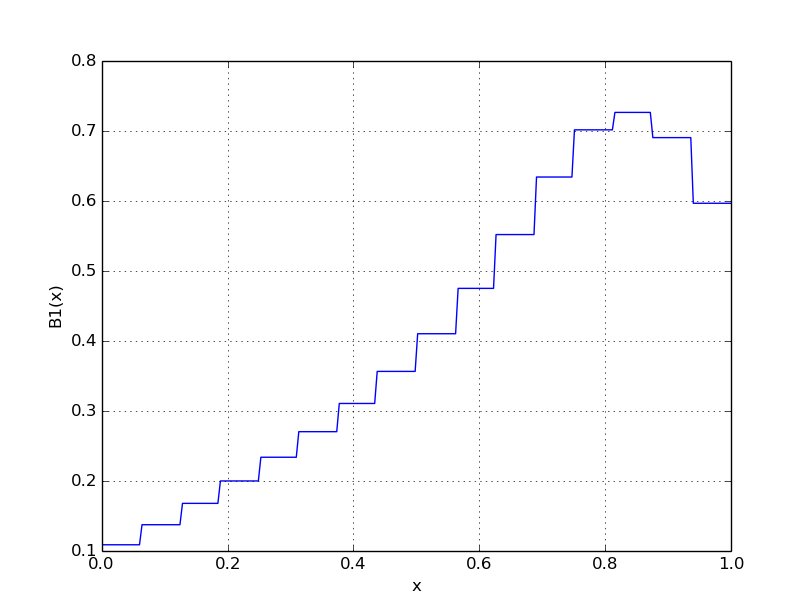
\includegraphics[width=6cm]{f1_025_haar_scale_b1_plot_n_16.png} }}%
    \qquad
    \subfloat[f1 025 haar scale b2 plot n 16]{{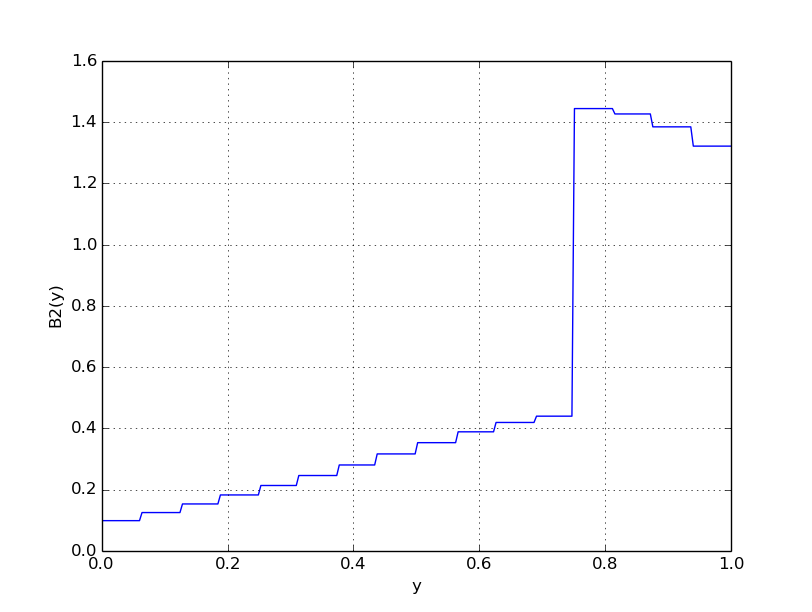
\includegraphics[width=6cm]{f1_025_haar_scale_b2_plot_n_16.png} }}%
    \caption{f1 025 haar scale n 16}%
    \label{fig:f1_025_haar_scale_plot_n_16}%
\end{figure}


\begin{figure}%
    \centering
    \subfloat[f1 025 llmw scale b1 plot n 16]{{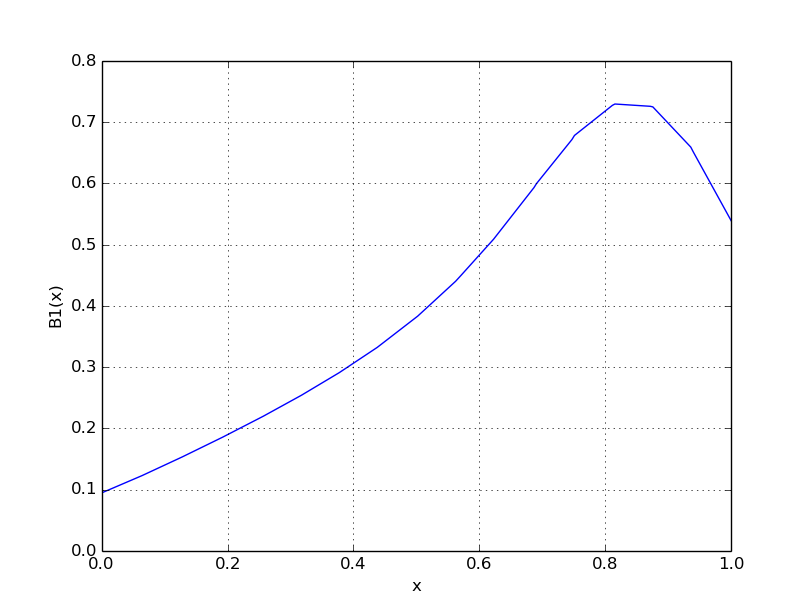
\includegraphics[width=6cm]{f1_025_llmw_scale_b1_plot_n_16.png} }}%
    \qquad
    \subfloat[f1 025 llmw scale b2 plot n 16]{{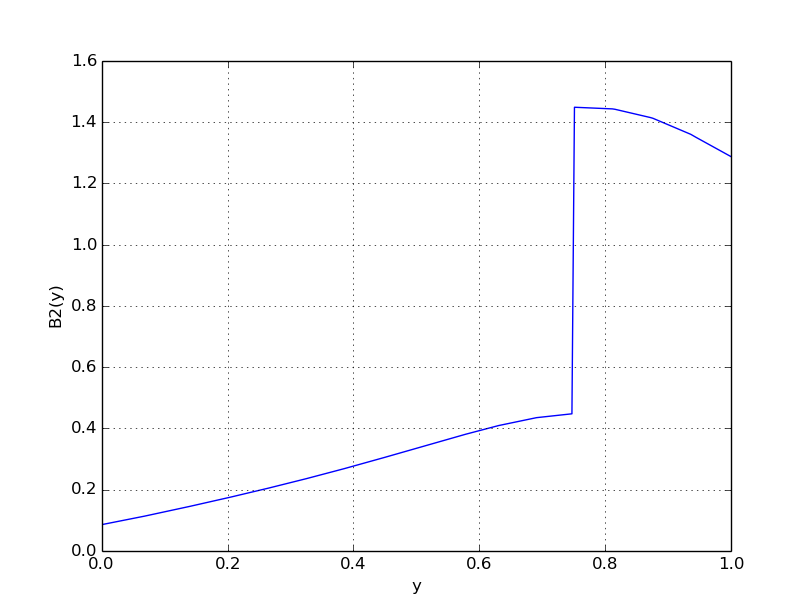
\includegraphics[width=6cm]{f1_025_llmw_scale_b2_plot_n_16.png} }}%
    \caption{f1 025 llmw scale n 16}%
    \label{fig:f1_025_llmw_scale_plot_n_16}%
\end{figure}


\begin{figure}%
    \centering
    \subfloat[f1 025 qlmw scale b1 plot n 16]{{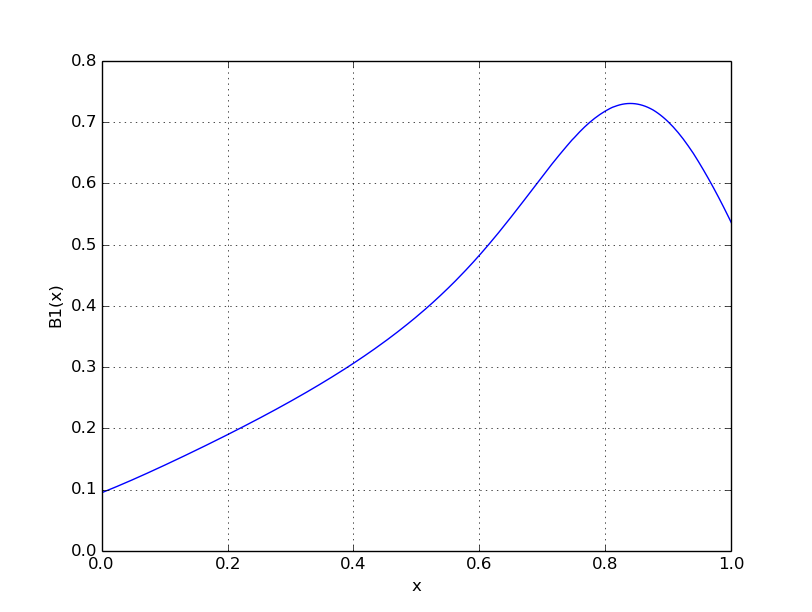
\includegraphics[width=6cm]{f1_025_qlmw_scale_b1_plot_n_16.png} }}%
    \qquad
    \subfloat[f1 025 qlmw scale b2 plot n 16]{{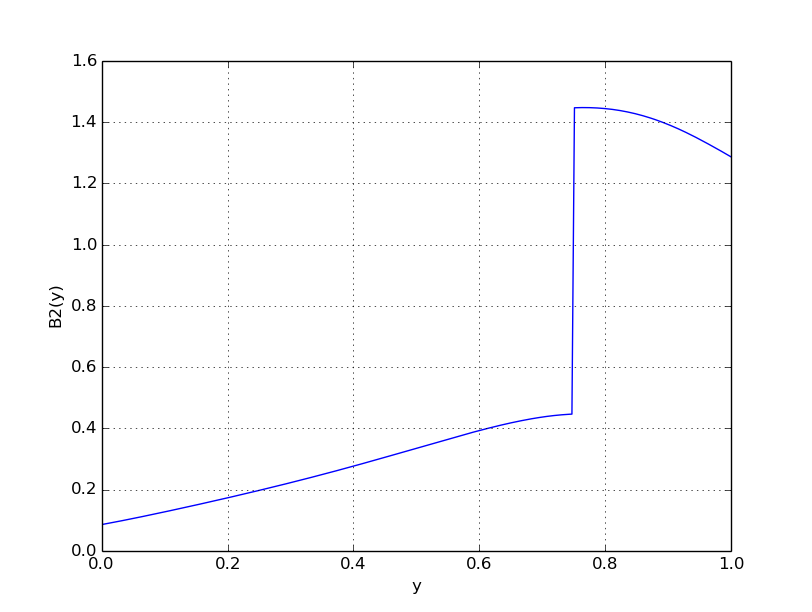
\includegraphics[width=6cm]{f1_025_qlmw_scale_b2_plot_n_16.png} }}%
    \caption{f1 025 qlmw scale n 16}%
    \label{fig:f1_025_qlmw_scale_plot_n_16}%
\end{figure}






\section{Three Dimensional Radiosity}
In this section we show results of projection method to solve 3D radiosity. Scene which we chose is, similar to Flatland scene 1, two square surface aligned and parallel to each other with light source on one of the surface as shown in Figure \ref{fig:3dparallel}. we divided each surface into grid of  $n*n$  sub-square elements of equal size and assumed the radiosity function, over the domain of surface, to be piecewise polynomial over each element. Thus we have projected radiosity function into space spanned by dilates and translates of two dimensional Wavelet basis. We use projection method discussed in Chapter \ref{ch:waveletprojection} to get system of linear equations which are solved to find the unknown projected function. Figure \ref{fig:3dhaar4},\ref{fig:3dhaar4} shows the solution and images of the scene for Haar wavelet with $n=4,16$. Similar to Haar wavelet we can use LLMW and QLMW for projection methods. In case of LLMW we are dealing with space of piecewise linear functions and LLMW wavelet forms the basis for the same space. In case of QLMW, we are dealing with space of piecewise quadratic function for which QLMW wavelet serves as alternative basis. See Figure \ref{fig:3dllmw4},\ref{fig:3dllmw16},\ref{fig:3dqlmw4}.
% Use of this alternative basis give us advantage of sparse matrix for which matrix inversion is faster. Figure \ref{}




\begin{figure}[tbh]
\centering{}
\captionsetup{justification=centering}
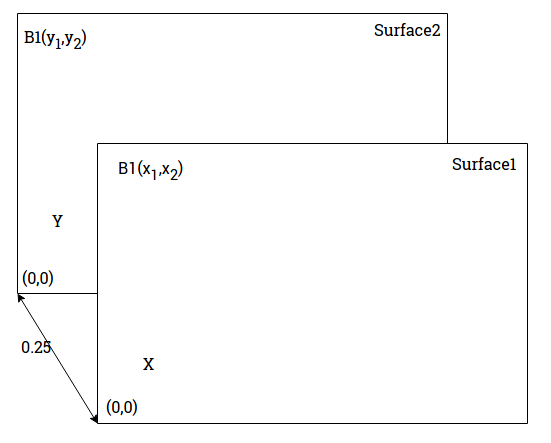
\includegraphics[width=5in]{3dparallel.png}
\caption{\label{fig:3dparallel}3D scene: Two parallel surfaces}
\end{figure}



\begin{figure*}
\centering
\subfloat[Image of Surface 1]{
\includegraphics[width=3in]{3dhaar4_025_1.png}
% \label{fig:llmwphi0}
}\subfloat[Image of Surface 2: With light source at center]{
\includegraphics[width=3in]{3dhaar4_025_2.png}
% \label{fig:llmwphi1}
}\\
\caption{\label{fig:3dhaar4}Solution of 3D scene with Haar wavelet and $n=4$}
\end{figure*}


\begin{figure*}
\centering
\subfloat[Image of Surface 1]{
\includegraphics[width=3in]{3dhaar16_025_1.png}
% \label{fig:llmwphi0}
}\subfloat[Image of Surface 2: With light source at center]{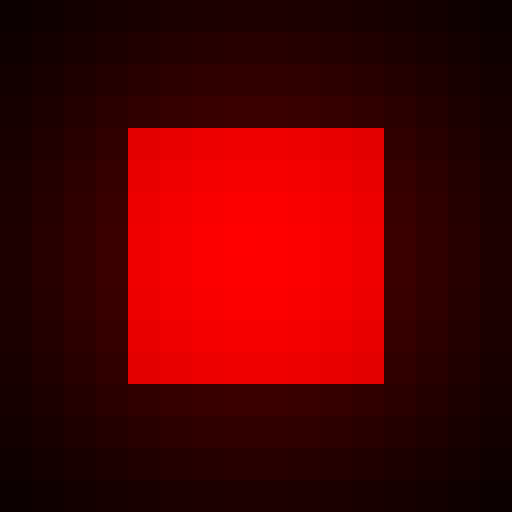
\includegraphics[width=3in]{3dhaar16_025_2.png}
% \label{fig:llmwphi1}
}\\
\caption{\label{fig:3dhaar16}Solution of 3D scene with Haar wavelet and $n=16$}
\end{figure*}



\begin{figure*}
\centering
\subfloat[Image of Surface 1]{
\includegraphics[width=3in]{3dhaar16_025_1.png}
% \label{fig:llmwphi0}
}\subfloat[Image of Surface 2: With light source at center]{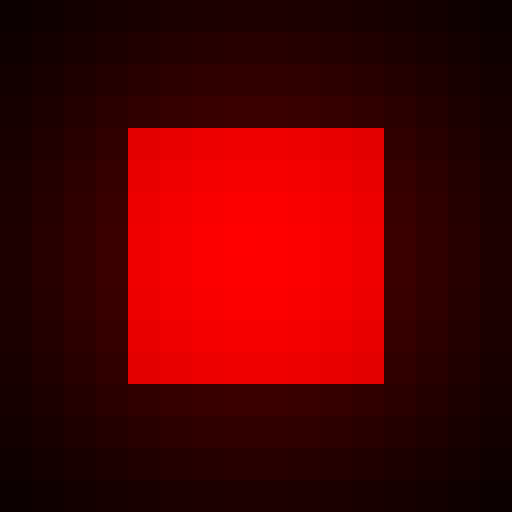
\includegraphics[width=3in]{3dhaar16_025_2.png}
% \label{fig:llmwphi1}
}\\
\caption{\label{fig:3dhaar16}Solution of 3D scene with Haar wavelet and $n=16$, retaining only half of the $256$ coefficients}
\end{figure*}





\begin{figure*}
\centering
\subfloat[Image of Surface 1]{
\includegraphics[width=3in]{3dllmw4_025_1.png}
% \label{fig:llmwphi0}
}\subfloat[Image of Surface 2: With light source at center]{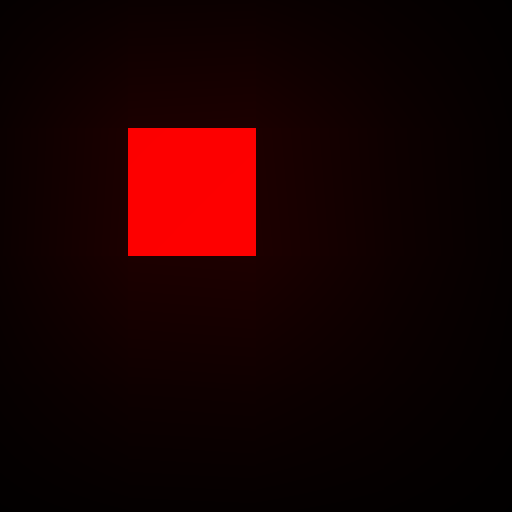
\includegraphics[width=3in]{3dllmw4_025_2.png}
% \label{fig:llmwphi1}
}\\
\caption{\label{fig:3dllmw4}Solution of 3D scene with LLMW wavelet and $n=4$}
\end{figure*}


\begin{figure*}
\centering
\subfloat[Image of Surface 1]{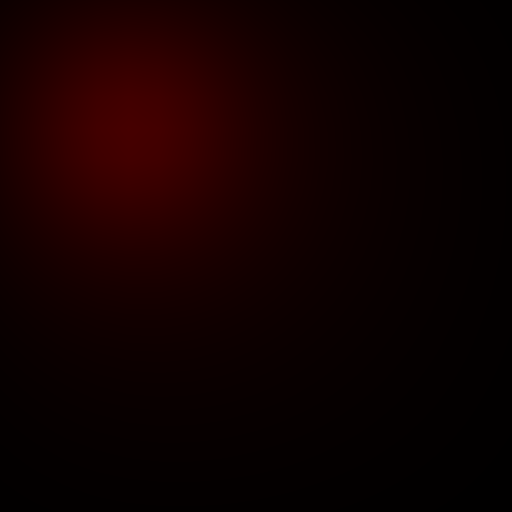
\includegraphics[width=3in]{3dllmw16_025_1.png}
% \label{fig:llmwphi0}
}\subfloat[Image of Surface 2: With light source at center]{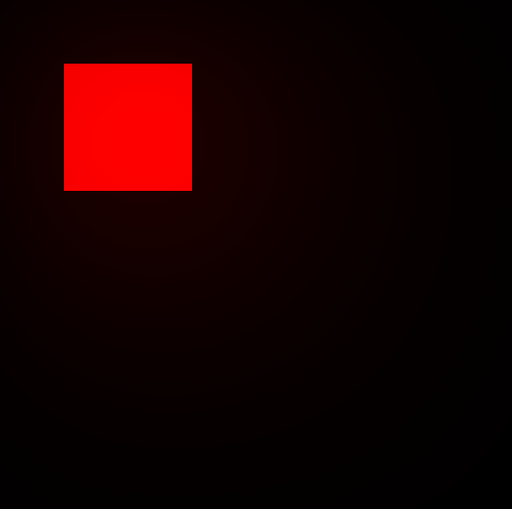
\includegraphics[width=3in]{3dllmw16_025_2.png}
% \label{fig:llmwphi1}
}\\
\caption{\label{fig:3dllmw16}Solution of 3D scene with LLMW wavelet and $n=16$}
\end{figure*}
\begin{figure*}
\centering
\subfloat[Image of Surface 1]{\includegraphics[width=3in]{3dllmw16_025_1.png}
% \label{fig:llmwphi0}
}\subfloat[Image of Surface 2: With light source at center]{\includegraphics[width=3in]{3dllmw16_025_2.png}
% \label{fig:llmwphi1}
}\\
\caption{\label{fig:3dllmw16}Solution of 3D scene with LLMW wavelet and $n=16$, retaining only quarter of the $1024$ coefficients}
\end{figure*}

\begin{figure*}
\centering
\subfloat[Image of Surface 1]{\includegraphics[width=3in]{3dqlmw4_025_1.png}
% \label{fig:qlmwphi0}
}\subfloat[Image of Surface 2: With light source at center]{\includegraphics[width=3in]{3dqlmw4_025_2.png}
% \label{fig:qlmwphi1}
}\\
\caption{\label{fig:3dqlmw4}Solution of 3D scene with QLMW wavelet and $n=4$}
\end{figure*}



\begin{figure*}
\centering
\subfloat[Image of Surface 1]{\includegraphics[width=3in]{3dqlmw4_025_1.png}
% \label{fig:qlmwphi0}
}\subfloat[Image of Surface 2: With light source at center]{\includegraphics[width=3in]{3dqlmw4_025_2.png}
% \label{fig:qlmwphi1}
}\\
\caption{\label{fig:3dqlmw4}Solution of 3D scene with QLMW wavelet and $n=4$, retaining only half of the $144$ coefficients}
\end{figure*}

% .\\\\\\\\\\\\{\bf flatland}\\

% {\bf 4d}\\
% \\section{Radiosity in three dimension} % (fold)
% \label{sec:radiosity_in_three_dimension}
% \underline{solution and threshold solution}
% % section radiosity_in_three_dimension (end)

    \chapter{conclusion and future work}
%\section{Appendix}
\begin{appendix}
\appendixpage
\chapter{}
\pagestyle{empty}
\section{\label{apen:derivationdegenerate}Fredholm IE and Derivation of Analytical Solution for Degenerate Kernel}
\label{appendix-1}

%\subsection{\label{apn: Matrix F}Frequency Variance Measure for Orthogonal Design}
Equation \ref{Freq. Var. matrix elements} has been derived in this section. The DTFT of the $h(n) \in l^2(\mathbb{Z})$  

\begin{equation}
H(\omega)=\sum^{M}_{n=0}h(n) e^{-j\omega n}
\end{equation}
Recall,
\begin{equation*}
h(n)=0 ,\, \forall n \in \{ (n < 0) \cup (n > M)\}
\end{equation*}
The DTFT of $h(n)$ can be rewritten in matrix form as:
\begin{equation}
H(\omega)=\mathbf{h}^{T}\mathbf{e}(\omega)
\end{equation}

where,

\begin{equation}
\mathbf{e}(\omega)=[e^{-j\omega}\,\,\,\ e^{-j\omega 1}\,\,\,\ e^{-j\omega 2}\,\,\,\,\ldots\,\,\,\ e^{-j\omega M}]^T
\end{equation}

The frequency variance $\sigma_{\omega}^{2}$ is given by

\begin{eqnarray}
\sigma_{\omega}^{2}&=&\frac{1}{\pi} \int_{0}^{\pi}\omega^{2} |H(\omega)|d\omega\\
&=&\frac{1}{\pi} \int_{0}^{\pi}\omega^{2} \{\mathbf{h}^{T}\mathbf{e}(\omega)\mathbf{e}^{H}(\omega)\mathbf{h}\}d\omega\\
&=&\mathbf{h}^{T}\{\int_{0}^{\pi}\omega^{2}\mathbf{e}(\omega)\mathbf{e}^{H}(\omega)\frac{d\omega}{\pi}\}\mathbf{h}\\
&=&\mathbf{h}^{T}\{\int_{0}^{\pi}\omega^{2}\mathbf{E}(\omega)\frac{d\omega}{\pi}\}\mathbf{h}\\
&=&\mathbf{h}^{T}\mathbf{F}\mathbf{h}
\end{eqnarray}
where,
\begin{equation}
\mathbf{F}=\int_{0}^{\pi}\omega^{2}\mathbf{E}(\omega)\frac{d\omega}{\pi}
\label{eq:F equation}
\end{equation}
and
\begin{eqnarray}
\mathbf{E}(\omega)&=&
\begin{bmatrix}
    e^{-j\omega 0}
\\ e^{-j\omega 1} 
\\ \vdots
\\ e^{-j\omega M}   
\end{bmatrix}
\begin{bmatrix}
    e^{j\omega 0}
& e^{j\omega 1} 
& \ldots
& e^{j\omega M}   
\end{bmatrix}\\
&=&
\begin{bmatrix}
1 & e^{j\omega 1}& e^{j\omega 2} & \ldots & e^{j\omega M}\\
e^{-j\omega 1} &  1& e^{j\omega 1} & \ldots & e^{j\omega (M-1)}\\
e^{-j\omega 2} & e^{-j\omega 1}& 1 & \ldots & e^{j\omega (M-2)}\\
\vdots & \vdots& \vdots & \ddots & \vdots\\
e^{-j\omega M} & e^{-j\omega (M-1)}& e^{-j\omega (M-2)} & \ldots & 1\\
\label{eq:E matrix}
\end{bmatrix}
\end{eqnarray}
The element of the $\mathbf{E}$ matrix is $E_{k,l} =e^{j\omega (l-k)}$.
So when $k=l$ the element at that place is 1 which means all the diagonal elements are 1.

Now consider the integral
\begin{equation*}
\frac{1}{\pi}\int_{0}^{\pi}\omega^{2} e^{j\omega p}d\omega
\end{equation*}\\

For p=0,
\begin{equation}
\frac{1}{\pi}\int_{0}^{\pi}\omega^{2} e^{j\omega p}d\omega=\frac{1}{\pi}\int_{0}^{\pi}\omega^{2}d\omega=\frac{\omega^3}{3\pi}\biggr\vert_{0}^{\pi}=\frac{\pi^2}{3}.
\label{eq:p=0}
\end{equation}\\
For $p>0$,
\begin{eqnarray*}
\frac{1}{\pi} \int_{0}^{\pi}\omega^{2} e^{j\omega p}d\omega &=& \frac{\omega^{2} e^{j\omega p}}{jp}\biggr\vert_{0}^{\pi}-\int_{0}^{\pi}\frac{2\omega e^{j\omega p}}{jp}d\omega \\
&=& \frac{\omega^{2} e^{j\omega p}}{jp}\biggr\vert_{0}^{\pi}-\frac{2}{jp}\int_{0}^{\pi} \omega e^{j\omega p}d\omega \\
&=&\frac{\omega^{2} e^{j\omega p}}{jp}\biggr\vert_{0}^{\pi}-\frac{2}{jp}\biggr\{ \frac{\omega e^{j\omega p}}{jp}\biggr\vert_{0}^{\pi}- \int_{0}^{\pi} \frac{ e^{j\omega p}}{jp}d\omega \biggr\}\\
&=&\frac{\omega^{2} e^{j\omega p}}{jp}\biggr\vert_{0}^{\pi}-\frac{2}{(jp)^{2}}\biggr\{ \omega e^{j\omega p}- \frac{ e^{j\omega p}}{jp} \biggr\}\biggr\vert_{0}^{\pi}\\
&=&\frac{\omega^{2} e^{j\omega p}}{jp}\biggr\vert_{0}^{\pi}+\frac{2}{(p)^{2}}\biggr\{ \omega e^{j\omega p}- \frac{ e^{j\omega p}}{jp} \biggr\}\biggr\vert_{0}^{\pi}\\
&=& \frac{\pi^{2}(-1)^{p}}{jp}+\frac{2}{p^2}\biggr\{\pi e^{j\pi p} - \frac{e^{j \pi p}}{jp}\biggr\}-\biggr[0+\frac{2}{p^2}\biggr(\frac{-1}{jp}\biggr)\biggr]\\
\end{eqnarray*}

Hence for $p>0$,
\begin{equation}
\frac{1}{\pi}\int_{0}^{\pi}\omega^{2} e^{j\omega p}d\omega= \frac{\pi^{2}(-1)^{p}}{jp}+\frac{2\pi (-1)^{ p}}{p^2}-\frac{2(-1)^p}{jp^3}+\frac{2}{jp^3}
\label{eq:p>0}
\end{equation}
From expressions \ref{eq:F equation}, \ref{eq:E matrix},\ref{eq:p=0} and \ref{eq:p>0}, we can evaluate the $\mathbf{F}$ matrix. The expression for the $\mathbf{F}$ matrix is given below.

 \begin{eqnarray}
 \label{Freq. Var. matrix}
 \mathbf{F_{k,l}} =  \begin{cases}
 \frac{\pi^2}{3}\,\,\, \text{if}\,\, k=l \\ 
 \frac{\pi^2{(-1)^{(l-k)}}}{j(l-k)} + \frac{2\pi{(-1)^{(l-k)}}}{(l-k)^2} + \frac{2\left(1 - {(-1)^{(l-k)}}\right)}{j{(l-k)^3}}\,\,\, \text{if}\,\, l \neq k
 \end{cases}
 \end{eqnarray}
\end{appendix}
    \bibliographystyle{plain}
    \bibliography{main}
    \thispagestyle{empty}
    

\end{document}
